%!TEX root = Manuscrit.tex
\chapter{Extension aux capteurs non-conventionnels}
\label{chap:extension}
\citationChap{I suppose it is tempting, if the only tool you have is a hammer, to treat everything as if it were a nail.}{Abraham Maslow}
\minitoc

\chapsummary{%
\lettrine{L}{es} images multispectrales sont couramment utilisées en télédétection, mais leur nombre de bandes élevé complique l'application directe de \glssymbol{FCN} préentraînés sur des données \gls{RVB}. Dans ce chapitre, nous montrons qu'il est en pratique tout de même possible d'étendre au cas multispectral les résultats obtenus en imagerie couleur. Nous étudions tout d'abord le cas d'images aériennes \gls{IRRVB}, avant d'adapter des \glssymbol{FCN} classiques pour la cartographie sémantique d'images multispectrales \glsname{Sentinel}-2, pour lesquelles la prise en compte des bandes non-visibles est largement bénéfique.

Nous nous intéressons ensuite au cas particulier de l'imagerie hyperspectrale, pour laquelle le nombre élevé de longueurs d'onde d'acquisition nécessite des précautions supplémentaires. Nous explorons les architectures des réseaux de l'état de l'art en apprentissage profond pour l'imagerie hyperspectrale et montrons qu'il existe un bénéfice significatif à déployer des modèles convolutifs à trois dimensions, en dépit du faible nombre d'exemples.

Enfin, nous étudions les possibilités de traitement des modèles numériques de terrain à partir de réseaux convolutifs. En effet, les modèles de terrain contiennent une information de hauteur particulièrement discriminante pour la végétation et les objets artificiels, absente des images orthorectifiées. Nous montrons que les \glssymbol{FCN} en niveaux de gris permettent d'obtenir des cartographies à partir de ces modèles, mais moins précises qu'en utilisant les images couleur, justifiant ainsi le besoin d'approches multimodales.
}

\newpage

\section{Images multispectrales}

Le chapitre précédent nous a permis de constater les excellentes performances des \glspl{FCN} pour la segmentation sémantique d'images aériennes \gls{RVB} et \gls{IRRV}. Toutefois, les satellites d'observation de la Terre, qu'ils soient institutionnels (\gls{Landsat}, \gls{SPOT}\dots) ou commerciaux (IKONOS, WorldView\dots), embarquent en grande majorité des capteurs \glslink{multispectral}{multispectraux}. Ces instruments permettent d'observer de l'information invisible pour l'\oe{}il humain dont il est désirable de tirer profit pour la cartographie automatisée.

\subsection{Prise en compte du proche infrarouge}

Les \glslink{multispectral}{capteurs multispectraux} les plus simples réalisent simultanément une acquisition couleur et infrarouge, formant ainsi des images à 4 canaux \gls{IRRVB}.
De nombreux satellites d'observation de la Terre en sont équipés, comme \gls{SPOT} et \gls{Pleiades} en France. En outre, ces satellites effectuent également une acquisition dite panchromatique dont la résolution spatiale est nettement supérieure. Cette combinaison est courante car les méthodes de super-résolution (\emph{pansharpening}) permettent de générer des images multispectrales à la résolution de l'image panchromatique. En première approche, nous pouvons considérer les images \gls{IRRVB} du jeu de données \gls{ISPRS} Potsdam qui présentent des propriétés similaires à celles attendues sur ces satellites.

Dans le~\cref{chap:cartographie}, nous avons établi que les \glspl{FCN} peuvent s'appliquer indifféremment aux images \gls{IRRV} et \gls{RVB} classiques. En particulier, nous avons été en mesure de transférer les poids de réseaux de préentraînés sur ImageNet à des images de télédétection \gls{IRRV}. Toutefois, ce transfert devient impossible dans le cas des images multispectrales \gls{IRRVB}, car la différence de nombre de canaux ne permet pas de conserver la topologie du réseau. Initialement, nous avons choisi de contourner ce problème en omettant le canal infrarouge et en ne considérant que les canaux visibles.

\begin{figure}[h]
  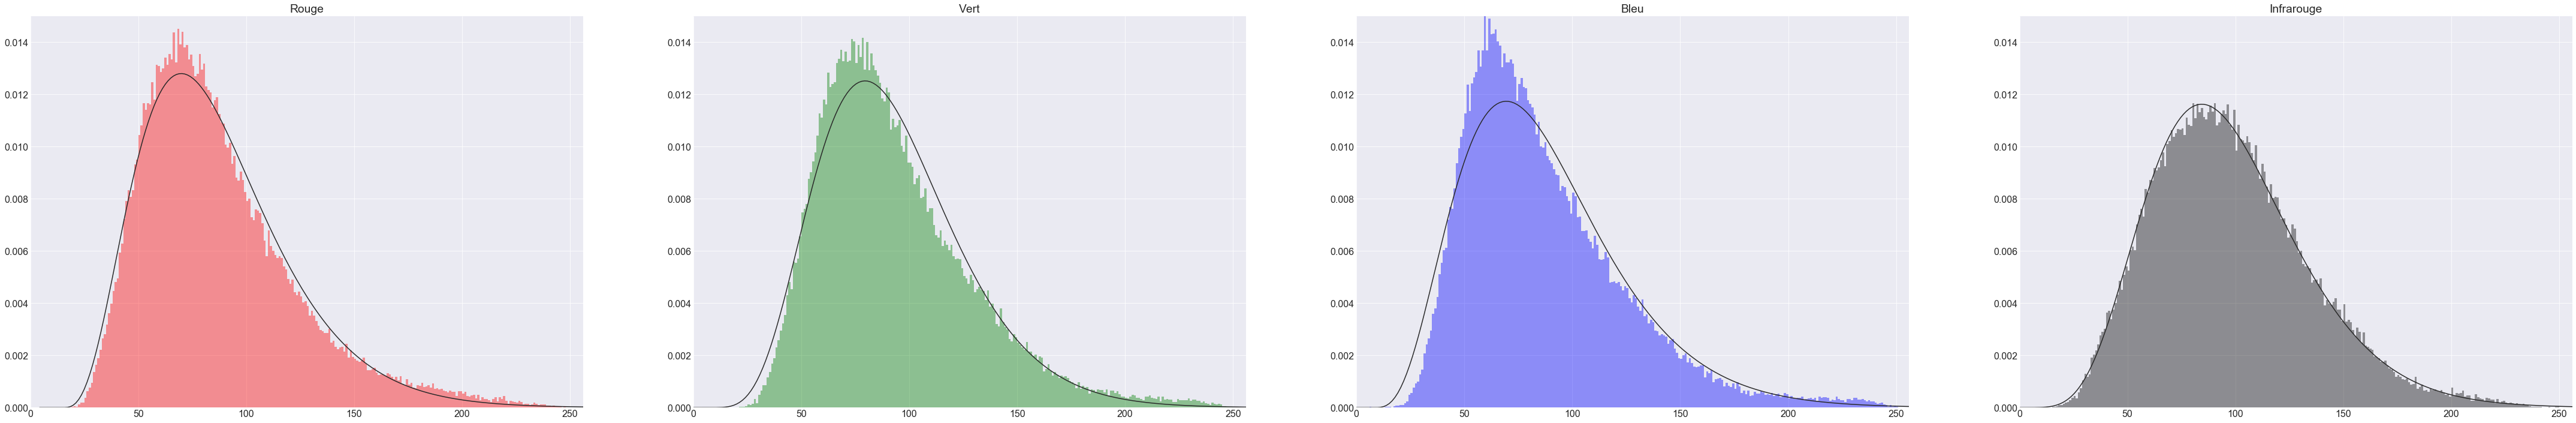
\includegraphics[width=\textwidth]{histogrammes_potsdam}
  \caption{Distributions des intensités pour les canaux rouge, vert, bleu et infrarouge du jeu de données \glssymbol{ISPRS} Potsdam.}
  \label{fig:potsdam_histograms}
\end{figure}

Avant toute expérimentation, nous pouvons examiner les distributions des intensités pour chaque canal au sein du jeu de données. Les histogrammes présentés dans la~\cref{fig:potsdam_histograms} révèlent que les distributions correspondent à des lois gamma dont les paramètres pour les canaux \gls{RVB} sont très proches. Néanmoins, les statistiques du canal infrarouge dévient significativement des canaux visibles, ce phénomène étant mis en évidence par les cartes de corrélation inter-canaux de la~\cref{fig:potsdam_correlations}. Les canaux visibles sont ainsi fortement corrélés (coefficient de Pearson supérieur à 0,87). À l'inverse, le canal infrarouge n'est que modérément corrélé avec les autres canaux, notamment lorsque l'écart en longueur d'onde s'accroît. Ainsi, le coefficient de Pearson entre les canaux rouge et infrarouge est de \num{0,80}, mais descend à \num{0,69} entre vert et infrarouge et \num{0,57} entre bleu et infrarouge.

\begin{figure}[h]
  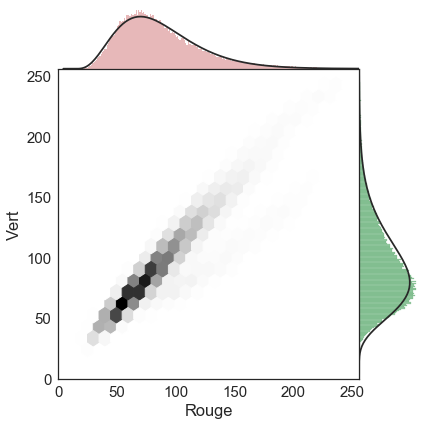
\includegraphics[width=0.33\textwidth]{hexbin_potsdam_rg}
  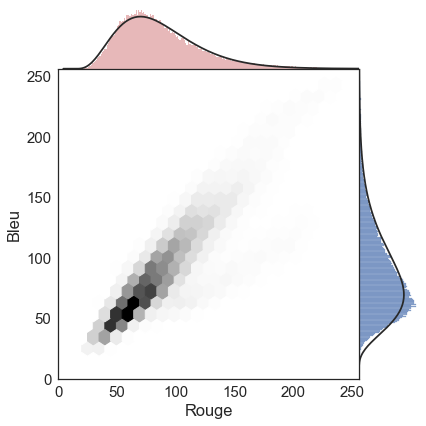
\includegraphics[width=0.33\textwidth]{hexbin_potsdam_rb}
  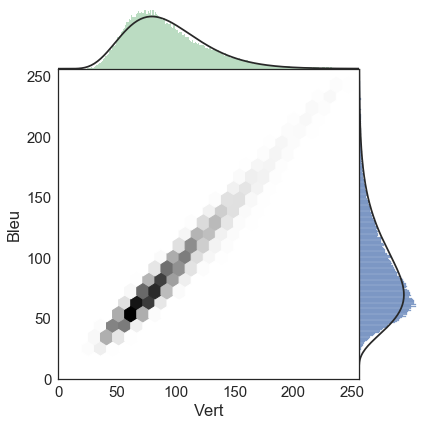
\includegraphics[width=0.33\textwidth]{hexbin_potsdam_gb}\\
  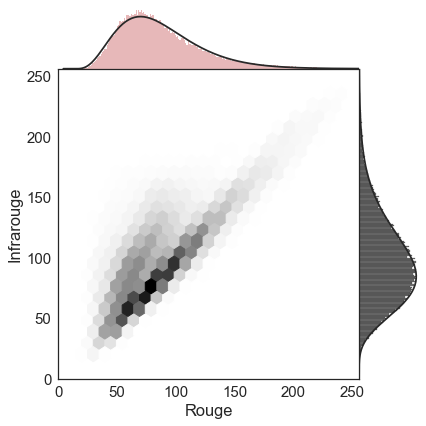
\includegraphics[width=0.33\textwidth]{hexbin_potsdam_rir}
  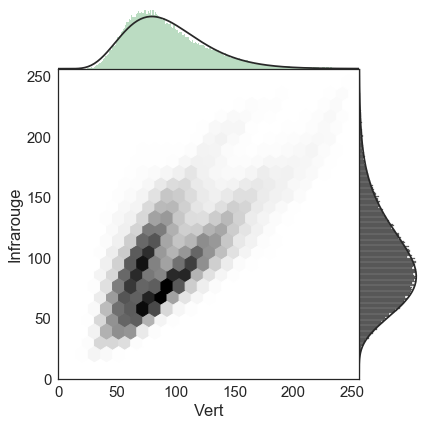
\includegraphics[width=0.33\textwidth]{hexbin_potsdam_gir}
  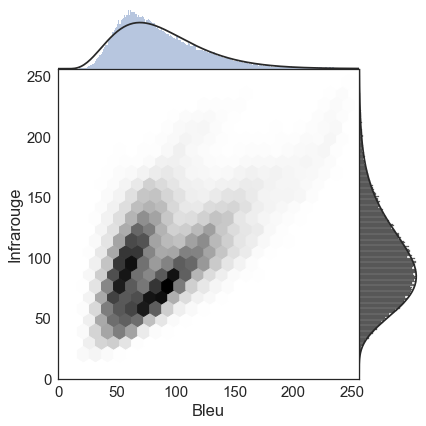
\includegraphics[width=0.33\textwidth]{hexbin_potsdam_bir}
  \caption{Cartes de corrélation entre canaux du jeu de données \glssymbol{ISPRS} Potsdam.}
  \label{fig:potsdam_correlations}
\end{figure}

Nous réalisons une étude préliminaire sur le jeu de données \glssymbol{ISPRS} Potsdam en reprenant les modèles et hyperparamètres décrits dans le~\cref{chap:cartographie}. En particulier, nous générons plusieurs variantes de \gls{SegNet}, avec et sans initialisation de l'encodeur à partir des poids de VGG-16 préentraîné sur ImageNet, pour différentes combinaisons de canaux. Cela nous permet d'isoler d'une part les variations de performances dues aux bandes spectrales et d'autre part celles provoquées par le transfert de connaissances depuis ImageNet. Les tuiles 2\_10, 2\_11, 2\_12, 3\_10, 3\_11, 3\_12, 4\_10, 4\_12, 5\_11, 5\_12, 6\_7, 6\_8, 6\_9, 6\_10, 6\_11, 7\_9, 7\_10 et 7\_12 sont utilisées pour l'entraînement tandis que la validation s'effectue sur les tuiles 4\_11, 5\_10, 6\_12, 7\_7, 7\_8 et 7\_11. Les résultats de cette expérience sont compilés dans le~\cref{tab:comparaison_bandes}.

\begin{table}
  \setlength\tabcolsep{3pt}
  \mycaption{Comparaison des performances de segmentation sémantique de SegNet sur le jeu de données de validation \glssymbol{ISPRS} Potsdam pour différentes combinaisons de canaux.}{Le transfert correspond à une initialisation à partir des poids entraînés sur ImageNet.}
  \label{tab:comparaison_bandes}
  \begin{tabularx}{\textwidth}{Y Y c c c c c c c}
    \toprule
    Canaux          & Transfert  & Routes        & Bâtiments     & Vég. basse    & Arbres        & Véhicules     & Autres        & Exactitude\\
    \midrule
    IR+B            & \Xmark            & \num{72.79}   & \num{87.22}   & \num{57.61}   & \num{71.74}   & \num{87.05}   & \num{13.15}   & \num{70.69}\\
    R+G             & \Xmark            & \num{89.92}   & \num{95.80}   & \num{81.49}   & \num{84.30}   & \num{95.21}   & \num{40.42}   & \num{88.48}\\
    IR+R            & \Xmark            & \num{90.75}   & \num{95.89}   & \num{82.77}   & \num{84.97}   & \num{95.50}   & \num{42.47}   & \num{89.25}\\
    \glsname{RVB}   & \Xmark            & \num{90.40}   & \num{96.32}   & \num{82.38}   & \num{83.78}   & \num{95.42}   & \num{39.97}   & \num{89.02}\\
    \glsname{IRRV}  & \Xmark            & \num{90.83}   & \num{95.91}   & \num{83.31}   & \num{84.26}   & \num{94.99}   & \num{43.74}   & \num{89.29}\\
    \glsname{IRRVB} & \Xmark            & \num{89.67}   & \num{95.57}   & \num{82.35}   & \num{83.82}   & \num{95.17}   & \num{42.89}   & \num{88.51}\\
    \glsname{RVB}   & \checkmark        & \num{92.35}   & \bres{97.62}{}& \num{85.18}   & \num{87.19}   & \bres{96.11}{}& \bres{52.15}{}& \num{91.22}\\
    \glsname{IRRV}  & \checkmark        & \bres{92.51}{}& \num{97.34}   & \bres{85.68}{}& \bres{87.54}{}& \bres{96.11}{}& \num{50.24}   & \bres{91.28}{}\\
    \bottomrule
  \end{tabularx}
\end{table}

En premier lieu, il apparaît que le choix des 3 canaux \gls{RVB} ou \gls{IRRV} n'a que peu d'influence sur les performances de classification du modèle. Cependant, la prise en compte de l'infrarouge au sein d'un modèle à quatre canaux \gls{IRRVB} dégrade significativement les résultats finaux. Ceci se vérifie également lorsque les poids des convolutions sont initialisés aléatoirement, c'est-à-dire sans préentraînement. Les résultats de classification des modèles entraînés sur 2 canaux seulement font apparaître une interaction négative entre les canaux infrarouge et bleu, entraînant une baisse conséquente des performances du modèle. Il semble ainsi y avoir un lien entre la cohérence radiométrique des canaux utilisés en entrée du réseau et la qualité finale de la classification. Ce lien est toutefois encore hypothétique et n'est pas trivial à mettre en évidence.

\subsection{Images multispectrales}
\label{sec:multispectral}

La majorité des capteurs optiques embarqués dans des satellites d'observation de la Terre opèrent en multispectral. En effet, l'information intéressante ne se situe pas toujours dans le domaine visible. La réponse lumineuse de la chlorophylle dans l'infrarouge proche est par exemple un indicateur caractéristique de la végétation invisible pour l'humain. Les longueurs d'onde d'acquisition supplémentaires permettent ainsi d'identifier des matériaux spécifiques qu'il est impossible de détecter autrement. L'instrumentation de \gls{Sentinel}-2 est conçue pour pouvoir détecter aussi bien les aérosols côtiers (bande 1 à \SI{443}{\nano\meter}), que le \emph{red edge} de la chlorophylle (bandes 5 à 7 entre \SI{705}{\nano\meter} et \SI{783}{\nano\meter}), la vapeur d'eau (bande 9 à \SI{945}{\nano\meter}) et les cirrus (bande 10 à \SI{1,375}{\micro\meter}). Les capteurs comportent, de par leur conception, une part de connaissance experte qu'il serait fâcheux d'ignorer.

Cette section s'intéresse donc à l'utilisation des \glspl{FCN} pour la segmentation sémantique d'images satellites multispectrales. Pour ce faire, nous tirons parti d'un ensemble d'images Sentinel-2 accompagné des cartes d'occupation des sols \emph{GlobeCover} 2009~\cite{arino_global_2012} fourni par~\citet{ben_hamida_deep_2017}. Les images Sentinel-2 considérées couvrent une région se situant à la frontière de la France, de la Suisse et de l'Italie et ont été acquises entre mai et octobre 2016. Nous faisons l'hypothèse que les changements d'occupation des sols durant les 7 années séparant la création de la carte et l'acquisition des données sont peu nombreux relativement à la surface couverte.

Un premier jeu de données est constitué à partir des images de mai à octobre ne contenant aucune couverture nuageuse (nuages opaques ou cirrus). Le second jeu de données comporte l'ensemble des images, y compris en présence de nuages, mais est restreint temporellement à la période estivale (juin à août). Dans ce deuxième cas, les nuages sont considérés comme une classe additionnelle à segmenter, à partir du masque fourni par le programme Copernicus. Les nuages sont en effet un problème majeur pour les capteurs optiques, la lumière ne pouvant les traverser sans une atténuation significative. Leur prise en compte est un enjeu considérable car il s'agit d'une occlusion souvent présente dans la plupart des zones climatiques. Les deux jeux de données comportent ainsi différentes acquisitions sur les mêmes zones à plusieurs dates. Les tuiles Sentinel-2 sont interpolées à une résolution de \SI{20}{\meter/\px} pour l'ensemble des bandes. Les annotations issues de \emph{GlobeCover} sont conservées à leur résolution originale de \SI{300}{\meter/\px}. Les~\cref{tab:datasets,tab:globecover_legende} récapitulent les propriétés des deux jeux de données et la liste des classes considérées.

\begin{table}[h]
\mycaption{Descriptifs des deux jeux de données d'images Sentinel-2 considérés.}{Le premier s'étend sur une longue période mais exclut les images contenant une couverture nuageuse. Le second est restreint à une période temporelle plus courte mais inclut les images en présence de nuages. Les deux jeux de données contiennent environ 150 millions de pixels chacun.}
\label{tab:datasets}
\begin{tabular}{lccc}
\toprule
Jeux de données & \multicolumn{3}{c}{nombre d'images}\\
(période)  & entraînement & validation  & nombre de classes \\
\midrule
D1, période longue sans nuage & & & \\
 (mai--oct. 2016) & 140 & 54 & 16 \\
\midrule
D2, période courte avec nuages & & & \\
(juin--août 2016) & 158 & 39 & 17 \\
\bottomrule
\end{tabular}
\end{table}

\begin{table}[h]
  \mycaption{Liste des classes des jeux de données D1 et D2 dérivées de \emph{GlobeCover} 2009.}{\small * La classe nuage est ajoutée \emph{a posteriori} à partir du masque fourni avec les données Sentinel-2 par Copernicus.}
  \label{tab:globecover_legende}
  \begin{tabularx}{\textwidth}{ccY}
    \toprule
    Valeur & Couleur        & Légende \emph{GlobeCover} 2009\\
    \midrule
    1 & \mybox{0,0,255}     & Cultures non irriguées\\ % Rainfeld croplands
    2 & \mybox{0,255,255}   & Mosaïque culture (50-70\%)/végétation (pelouse, fruticée, forêt) (20-50\%)\\ % Mosaic Cropland (50-70%) / Vegetation (grassland, shrubland, forest) (20-50%)
    3 & \mybox{0,255,0}     & Mosaïque végétation (pelouse, fruticée, forêt) (50-70\%)/cultures (20-50\%)\\ % Mosaic Vegetation (grassland, shrubland, forest) (50-70%) / Cropland (20-50%)
    4 & \mybox{255,0,0}     & Forêt décidue à feuilles larges dense (>40\%, >5m)\\ %Closed (>40%) broadleaved deciduous forest (>5m)
    5 & \mybox{128,0,0}     & Forêt épineuse sempervirent dense (>40\%, >5m)\\ %Closed (>40%) needleleaved evergreen forest (>5m)
    6 & \mybox{0,128,0}     & Forêt peu dense (15-40\%) décidue ou sempervirent (>5m)\\%Open (15-40%) needleleaved deciduous or evergreen forest
    7 & \mybox{0,0,128}     & Forêt mixe décidue et sempervirent peu dense (>15\%, >5m)\\%Closed to open (>15%) mixed broadleaved and needleleaved forest (>5m)
    8 & \mybox{128,128,128} & Mosaïque forêt et fruticée (50-70\%)/pelouse (20-50\%)\\%Mosaic Forest/Shrubland (50-70%) / Grassland (20-50%)
    9 & \mybox{128,128,0}   & Mosaïque pelouse (50-70\%)/forêt et fruticée (20-50\%)\\%Mosaic Grassland (50-70%) / Forest/Shrubland (20-50%)
    10 & \mybox{128,0,128}  & Fruticée peu dense (>15\%, <5m)\\%Closed to open (>15%) shrubland (<5m)
    11 & \mybox{0,128,128}  & Pelouse peu dense (>15\%)\\%Closed to open (>15%) grassland
    12 & \mybox{64,0,0}     & Végétation éparse (boisée, fruticées, pelouse, >15\%)\\%Sparse (>15%) vegetation (woody vegetation, shrubs, grassland)
    13 & \mybox{64,64,64}   & Végétation peu dense (boisée, fruticées, pelouse) sur sol régulièrement inondé ou détrempé (eau douce, saumâtre ou salée)\\%Closed to open (>15%) vegetation (grassland, shrubland, woody vegetation) on regularly flooded or waterlogged soil - Fresh, brackish or saline water
    14 & \mybox{64,64,0}    & Surface artificielle ou assimilée (urbanisation>50\%)\\%Artificial surfaces and associated areas (urban areas >50%)
    15 & \mybox{0,64,64}    & Zone de terre nue\\%Bare areas
    16 & \mybox{64,0,64}    & Étendue d'eau\\%Water bodies
    17 & \mybox{0,0,0}      & Nuage*\\%Clouds
    \bottomrule
  \end{tabularx}
\end{table}

Afin de réaliser la segmentation sémantique sur ces images, nous considérons une architecture SegNet réduite, dont le décodeur est coupé après le deuxième bloc convolutif. En effet, il ne nous est pas utile d'obtenir des cartes à résolution $1:1$. Nous utilisons donc l'approche multiéchelle de la~\cref{sec:deep_multiscale} pour générer des cartes à résolution $1:8$ (\SI{160}{\meter/\px}), $1:16$ et $1:32$. Ceci diminue à la fois le temps de calcul et le nombre de paramètres à optimiser. Les cartes sont finalement interpolées à \SI{300}{\meter/\px} puis moyennées avant le calcul du \emph{softmax}. La prédiction finale est comparée à la vérité terrain durant l'entraînement en utilisant l'entropie croisée.

Nous comparons pour cette tâche deux variantes de SegNet. La première, SegNet \gls{RVB}, n'opère que sur les bandes 2,3 et 4 de Sentinel-2 correspondant à une image en vraies couleurs. La deuxième, SegNet \glslink{multispectral}{MSI}, est entraînée sur l'ensemble des 12 bandes\footnote{La bande 8A n'est pas utilisée.}. Les hyperparamètres restants sont repris du~\cref{chap:cartographie}. Les réseaux sont optimisés jusqu'à convergence par descente de gradient stochastique avec moment, avec un taux d'apprentissage fixé à \num{0,001} et un moment de \num{0,9} pendant \num{150000} itérations. Les variantes \gls{RVB} et \glslink{multispectral}{MSI} utilisent respectivement une taille de \emph{batch} de 20 et 10, pour chacune occuper environ 6 Go de mémoire \gls{GPU}. L'entraînement prend environ 18 heures sur un \gls{GPU} NVIDIA Titan X (génération Pascal) à l'aide de notre implémentation \gls{PyTorch}~\cite{noauthor_pytorch_2016}.

Le modèle entraîné sur les 12 bandes atteint \num{66,5}\% d'exactitude sur le jeu de données D1 (sans nuage) et \num{86,4}\% sur D2 (avec nuages). L'écart important entre les jeux de données est une combinaison de deux facteurs. Tout d'abord, la présence des nuages nombreux et faciles à détecter (score $F_1 > 97\%$) augmente statistiquement le nombre de pixels bien classifiés. Néanmoins, comme le montre le~\cref{tab:s2_results}, les performances sur l'ensemble des classes de D1 sont inférieures à celles des mêmes classes sur D2. Ceci s'explique par la faible variabilité des images de D1. Ce jeu de données ayant été constitué sous contrainte d'une couverture nuageuse faible, son étendue spatiale est plus faible et les conditions environnementales sont moins variées. Les modèles appris sur D1 généralisent donc moins bien sur les nouvelles acquisitions. À l'inverse, D2 couvre une période temporelle faible mais avec de nombreuses variations environnementales et donc une variété d'images plus importante. Cela permet au modèle d'apprendre les invariants radiométriques nécessaires à une bonne généralisation.
Enfin, la prise en compte de l'ensemble des 12 bandes multispectrales permet de gagner 2\% d'exactitude sur D1 et \num{2,5}\% sur D2 par rapport au modèle \gls{RVB} seul. Ce phénomène n'est pas lié à une classe en particulier, puisque la majorité d'entre elles bénéficient des bandes spectrales additionnelles (cf.~\cref{tab:s2_results}). Ceci conforte notre intuition initiale\,: l'information multispectrale est plus riche et plus discriminante que l'image couleur.

Il nous paraît indispensable de souligner que les annotations considérées proviennent d'une source ancienne (2009) et grossière (\SI{300}{\meter/\px}). Cela explique notamment l'apparence pixellisée de la vérité terrain sur les illustrations, qui introduit une approximation dans le protocole d'évaluation. En effet, les scènes observées par Sentinel-2 peuvent avoir changé de type d'occupation des sols depuis 2009. En outre, la résolution de Sentinel-2 permet d'identifier des objets et des structures qui étaient mélangées, et donc invisibles, dans \emph{GlobeCover}. Toutefois, l'adéquation géométrique entre les prédictions et la vérité terrain est visuellement forte. Il est plausible que certains désaccords entre le modèle et les annotations soient en réalité dus à la nature approximative de \emph{GlobeCover} et aux changements temporels, et que les prédictions faites par SegNet soient en réalité plus précises sur certaines classes -- notamment les surfaces artificialisées -- que la vérité terrain dont nous disposons. Les~\cref{fig:segnet_msi_d1,fig:segnet_msi_d2} illustrent quelques exemples qualitatifs de cartes générées par nos modèles.

Finalement, cette étude nous permet d'aboutir à deux conclusions. D'une part, elle montre la pertinence des modèles entièrement convolutifs pour le traitement des images multispectrales. En effet, l'architecture SegNet s'étend avec succès aux données Sentinel-2. S'il est nécessaire d'arbitrer certains choix techniques, notamment concernant l'interpolation des bandes et le choix d'une résolution de référence pour la vérité terrain, il ne semble pas y avoir de verrou majeur à l'utilisation des \glspl{FCN} pour les données multispectrales. D'autre part, l'inclusion des bandes hors du domaine visible permet d'augmenter l'expressivité du modèle, qui bénéficie de la richesse de l'information multispectrale. Cela permet notamment d'améliorer le pouvoir discriminant du SegNet sur des classes pouvant être ambiguës en \gls{RVB}.

\begin{table}[h]
  \mycaption{Performances de SegNet sur les jeux de données D1 et D2 Sentinel-2}{(cf.~\cref{tab:globecover_legende} pour le détail des classes).}
  \label{tab:s2_results}
  \setlength\tabcolsep{2pt}
  \scalebox{0.75}[0.75]{
  \begin{tabularx}{1.33\textwidth}{Yccccccccccccccccccc}
    \toprule
    Jeu de données      &  Modèle                     & Exactitude & 1    & 2    & 3    & 4    & 5    & 6    & 7    & 8    & 9    & 10   & 11   & 12   & 13   & 14   & 15   & 16   & 17  \\
    \midrule
    \multirow{2}{*}{D1} &  SegNet \glsname{RVB}             & \num{55,0} & \num{39.0} & \num{35.5} & \num{1.81} & \num{71.0} & \num{0.91} & \num{0.00} & \num{0.00} & \num{0.00} & \num{0.00} & \num{2.08} & \num{0.00} & \num{5.33} & \num{0.00} & \num{36.0} & \num{0.00} & \num{74.6} & --\\
                        &  SegNet \glssymbol{multispectral} & \num{66,5} & \num{36.2} & \num{38.1} & \num{1.45} & \num{85.1} & \num{6.33} & \num{0.00} & \num{1.39} & \num{0.00} & \num{0.00} & \num{2.18} & \num{0.00} & \num{3.36} & \num{0.00} & \num{34.3} & \num{0.00} & \num{97.8} & --\\
    \midrule
    \multirow{2}{*}{D2} &  SegNet \glsname{RVB}             & \num{84,9} & \num{74,7} & \num{64,1} & \num{38,0} & \num{89,9} & \num{68,4} & \num{58,4} & \num{51,4} & \num{36,7} & \num{39,8} & \num{61,0} & \num{45,7} & \num{55,2} & \num{47,9} & \num{76,9} & \num{66,9} & \num{98,7} & \num{96,7}\\
                        &  SegNet \glssymbol{multispectral} & \num{86,4} & \num{76,0} & \num{66,8} & \num{43,4} & \num{92,4} & \num{72,3} & \num{51,0} & \num{59,5} & \num{22,9} & \num{50,0} & \num{67,4} & \num{48,0} & \num{53,5} & \num{41,0} & \num{77,0} & \num{66,7} & \num{98,8} & \num{97,7}\\
    \bottomrule
  \end{tabularx}}
\end{table}

\begin{figure}[h]
  \foreach\idx in {3,2}{
  \begin{subfigure}{\textwidth}
    \foreach\picname\picpath in {Couleur naturelle/sentinel_rgbclouds_\idx_tci,
                                 Prédiction/sentinel_rgbclouds_\idx_pred,
                                 Vérité terrain/sentinel_rgbclouds_\idx_gt}{
    \begin{subfigure}{0.33\textwidth}
      \includegraphics[width=\textwidth]{\picpath}
      \caption*{\picname}
    \end{subfigure}}%
  \end{subfigure}}
  \caption{Exemples de prédictions du modèle SegNet \glslink{multispectral}{MSI} entraîné sur D2 (avec nuages).}
  \label{fig:segnet_msi_d2}
\end{figure}

\begin{figure}[h]
  \foreach\picname\picpath in {Couleur naturelle/sentinel_rgbnoclouds_tci,
                               Prédiction/sentinel_rgbnoclouds_pred,
                               Vérité terrain/sentinel_rgbnoclouds_gt}{
  \begin{subfigure}{0.33\textwidth}
    \includegraphics[width=\textwidth]{\picpath}
    \caption*{\picname}
  \end{subfigure}}%
  \caption{Exemples de prédictions du modèle SegNet \glslink{multispectral}{MSI} entraîné sur D1 (sans nuage).}
  \label{fig:segnet_msi_d1}
\end{figure}

\section{Imagerie hyperspectrale}

\begin{figure}
  \begin{minipage}[t]{0.485\textwidth}
      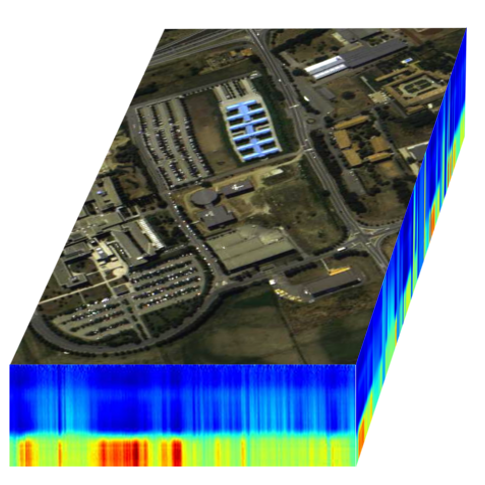
\includegraphics[width=\textwidth]{hyperspectral_cube_pavia}
      \caption{Exemple de cube hyperspectral sur le jeu de données \emph{Pavia University}.}
      \label{fig:cube_hyperspectral}
  \end{minipage}
  \hfill
  \begin{minipage}[t]{0.485\textwidth}
      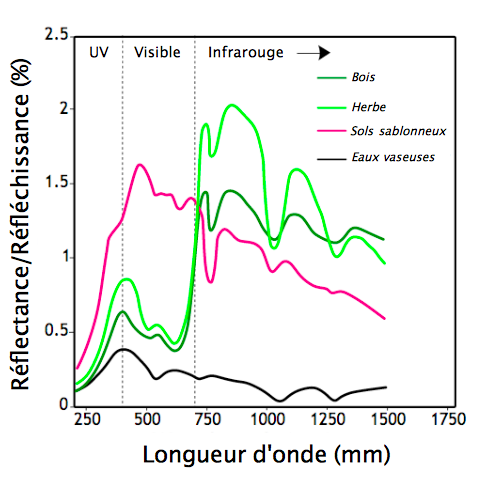
\includegraphics[width=\textwidth]{reflectances}
      \caption{Exemple de réflectances caractéristiques de diverses surfaces terrestres.}
      \small{Crédits image\,: \href{https://commons.wikimedia.org/wiki/File:R\%C3\%A9flectance_surfaces_terrestres.png}{Arbeck (Wikimedia Commons, CC-BY-SA 3.0)}}
      \label{fig:reflectances}
  \end{minipage}
\end{figure}

Jusqu'ici, nous avons pu constater que l'interprétation d'images couleur \gls{RVB} et infrarouges classiques bénéficie considérablement de l'introduction des \glslink{CNN}{réseaux de neurones convolutifs profonds}. Qui plus est, la~\cref{sec:multispectral} nous a permis d'étendre les \glspl{CNN} au cas \glsname{multispectral} et d'exploiter à bon escient les longueurs d'onde supplémentaires afin d'identifier des objets indétectables précédemment. En réalité, chaque matériau possède une signature spectrale caractéristique définie par la façon dont il réfléchit la lumière. Il paraît donc naturel de chercher à acquérir simultanément la réponse en intensité sur l'ensemble du spectre lumineux afin de réaliser une analyse fine des surfaces~\cite{cubero-castan_physics-based_2015,fabre_estimation_2015}.

Cette logique est à l'origine du développement des capteurs \glslink{hyperspectral}{hyperspectraux}. Ceux-ci possèdent une faible résolution spatiale, mais une très grande résolution spectrale et sont capables de mesurer la réponse lumineuse d'un objet sur plusieurs centaines de bandes spectrales régulièrement espacées. Les méthodes de \emph{deep learning} purement orientées vision ne peuvent pas se transposer directement à de telles données. En effet, la dimension spectrale prédomine devant les dimensions spatiales caractéristiques des objets d'intérêt. À titre d'exemple, une acquisition hyperspectrale aérienne typique présentera une résolution au sol au mieux de \SI{1}{\meter/\px} et une résolution spectrale d'environ \SI{10}{\nano\meter/bande}, pour 200 bandes spectrales entre \SI{0,4}{\micro\meter} et \SI{2,5}{\micro\meter}. Si l'on considère une maison individuelle de \SI{12x10}{\meter} \footnote{D'après le ministère de l'environnement, la surface de plancher moyenne des maisons françaises était de \SI{121}{\meter\squared} en 2015 (\href{http://www.cohesion-territoires.gouv.fr/IMG/pdf/datalab-essentiel-51-le-prix-des-terrains-a-batir-en-2015-oct2016.pdf}{\og \emph{Le prix des terrains à bâtir en 2015\fg}}).}, cet objet en hyperspectral sera décrit par un tenseur de taille \num{12x10x200}.
En comparaison, les acquisitions aériennes \gls{RVB} en \gls{EHR} présentent une résolution spatiale de l'ordre de \SI{10}{\centi\meter/\px} sur 3 bandes entre \SI{0,4}{\micro\meter} et \SI{0,7}{\micro\meter}. La même maison serait alors caractérisée par un tenseur de dimensions $120\times100\times3$. Si le volume de données est similaire (\num{24000} scalaires contre \num{36000}), leur répartition est nettement différente. En pratique, on parle ainsi de cube hyperspectral, ou \emph{hypercube} (cf.~\cref{fig:cube_hyperspectral}). Enfin, compte-tenu de la faible résolution spatiale des capteurs hyperspectraux, un hypercube couvre une même zone avec moins de pixels qu'une image couleur. Le nombre d'échantillons annotés pour l'entraînement de modèles supervisés sera donc plus faible que précédemment. Ces deux propriétés sont les principaux obstacles auxquels nous allons faire face pour mettre en \oe{}uvre l'apprentissage profond sur des hypercubes.

La~\cref{sec:principes_hsi} rappelle les fondamentaux de l'imagerie hyperspectrale. La~\cref{sec:hyperspectral_datasets} détaille les jeux de données hyperspectraux mis à la disposition de la communauté scientifiques, tandis que la~\cref{sec:classif_hsi} réalise un bref tour d'horizon des approches de classification traditionnellement mises en \oe{}uvre sur ces images. Enfin, la~\cref{sec:deep_hsi} clôture cette partie avec une étude comparative, théorique et expérimentale, des modèles de réseaux profonds pour la cartographie à partir de données hyperspectrales. Le lecteur averti des spécificités liées à l'imagerie hyperspectrale pourra directement se diriger vers cette dernière section.

\subsection{Principes physiques de l'imagerie hyperspectrale}
\label{sec:principes_hsi}
%\textit{Paragraphe rédigé à partir d'éléments d'un mail de Xavier Ceamanos, ONERA.}

Physiquement, un capteur hyperspectral mesure\footnote{Les caméras multispectrales et hyperspectrales fonctionnent généralement sur un mode \emph{push broom} réalisant une acquisition ligne par ligne, différent des appareils photographiques habituels. Les détails techniques liés aux capteurs et à leur étalonnage ne seront pas abordés dans ce manuscrit.} l'intensité (en unité de luminance spectrale) du flux lumineux $\phi$ par unité de surface et par unité d'angle solide. Il s'agit d'une grandeur physique qui a pour unité le \si{\watt\per\square\meter\per\steradian}. Le capteur mesure ce flux lumineux sur un ensemble de bandes radiométriques régulièrement espacées, dont la largeur varie aux alentours de \SI{10}{\nano\meter}. Pour chaque pixel, c'est-à-dire pour chaque unité de surface, le capteur échantillonne ainsi la signature spectrale de la surface sur plusieurs centaines de longueurs d'onde. Chacun de ces spectres peut se représenter sous la forme d'une courbe de réponse spectrale comme celles de la~\cref{{fig:reflectances}}. Ce flux lumineux intègre la lumière émise et réfléchie par l'objet, mais aussi celle diffusée par l'environnement, qui s'ajoute à la mesure.

En observation de la Terre, les acquisitions sont réalisées depuis le sommet de l'atmosphère (en satellite) ou depuis l'atmosphère même (en aéroporté). Or, l'atmosphère n'est pas neutre et altère le signal lumineux lors de sa propagation. Les images satellitaires sont régulièrement perturbées par les nuages, les effets de brumes et les aérosols en suspension dans l'air. Compte-tenu de la finesse des bandes d'acquisition, les capteurs hyperspectraux sont particulièrement sensibles à ces phénomènes. En ce qui nous concerne, nous nous intéressons aux surfaces et aux matériaux présents sur le sol. La mesure pertinente est donc la réflectance du sol, définie comme le rapport entre le flux émis par celui-ci et le flux incident~:
\begin{equation}
  \rho = \frac{\phi_{\mathit{r\acute{e}fl\acute{e}chi}}}{\phi_\mathit{incident}}~~.
\end{equation}

La réflectance $\rho$ est un indicateur du pouvoir réfléchissant d'un objet pour une longueur d'onde donnée (on parle également d'albédo du matériau). C'est une grandeur sans unité comprise entre 0 (surface complètement absorbante) et 1 (surface totalement réfléchissante). En règle générale, un matériau renvoyant plus de 80\% de la lumière blanche apparaît blanc, tandis qu'un matériau réfléchissant moins de 3\% apparaît noir. Comme pour la luminance, on considère la réflectance radiométrique $\rho_\lambda$, qui varie en fonction de la longueur d'onde. La réflectance est préférée à la luminance car il s'agit d'une propriété intrinsèque au matériau, indépendante de l'environnement extérieur. La courbe de réflectance d'un matériau correspond de fait à une signature spectrale dotée d'un fort pouvoir discriminant~(cf.~\cref{fig:reflectances}). Lorsque c'est possible, on cherchera donc à travailler sur des données en réflectance.

\paragraph{Corrections environnementales}
Passer de la luminance à la réflectance nécessite d'éliminer l'influence de l'environnement sur l'intensité lumineuse mesurée par le capteur. La compensation des phénomènes perturbatoires impliquent des techniques dites de correction atmosphérique~\cite{deschamps_atmospheric_1980, rahman_smac_1994, chavez_image-based_1996}. Celles-ci permettent de réduire l'influence de l'atmosphère sur la mesure~\cite{gao_atmospheric_2009} et transforment les images de luminance en images de réflectance. Pour ce faire, les spécialistes conçoivent des modèles d'atmosphère qu'ils inversent afin d'estimer puis d'éliminer l'influence de la diffusion lumineuse et des phénomènes radiatifs. Généralement, ces modèles nécessitent de connaître les paramètres environnementaux tels que l'ensoleillement. Ces informations peuvent être obtenues a posteriori, grâce aux éphémérides, ou \emph{in situ} en embarquant un capteur d'ensoleillement sur le dos de l'appareil. Les capteurs hyperspectraux portatifs éclairent directement la cible et permettent ainsi de s'affranchir des conditions environnementales.

Par ailleurs, notons que le calcul de la réflectance se fait le plus souvent sous hypothèse de planarité du sol. Le relief naturel du terrain et la présence d'objets surélevés introduit en effet réflexions et occlusions indésirables. Les premières peuvent conduire à des sur-illuminations lorsque plusieurs réflexions convergent vers le même point, tandis que les secondes génèrent des ombres. Certaines techniques de correction incluent donc parfois le \gls{MNE} afin de prendre en compte la géométrie de la scène, notamment en milieu urbain~\cite{ceamanos_using_2017}.

Dans tous les cas, il est nécessaire de garder à l'esprit que toute correction, aussi maîtrisée soit-elle, est imparfaite et susceptible d'introduire des erreurs et des incertitudes dans les données.

\paragraph{Visualisation}
Contrairement à la vision humaine, la plage de fonctionnement d'une caméra hyperspectrale s'étend bien au-delà du domaine visible. La plupart des capteurs balaient les longueurs d'onde de l'ultra-violet (\SI{300}{\nano\meter}) jusqu'à la limite de l'infrarouge moyen (\SI{3 000}{\nano\meter}) par tranches de \SI{10}{\nano\meter}. En comparaison, le spectre visible ne couvre que les longueurs d'onde de \SI{300}{\nano\meter} à $\simeq$ \SI{700}{\nano\meter}. Les écrans de la vie courante utilisent le mode \gls{RVB} et produisent une image comme l'agrégation de trois cartes d'intensité en rouge, vert et bleu. Cette approche correspond aux trois types de récepteurs situés dans l'\oe{}il humain. Néanmoins, une image hyperspectrale correspond à un cube de données au sein duquel chaque pixel contient une réponse spectrale complète. Ces signatures spectrales caractérisent les surfaces et les matériaux lorsqu'ils sont purs. En pratique, la faible résolution spatiale implique que le spectre mesuré pour un pixel soit un mélange de différents matériaux, d'autant plus dans le cas de la végétation.

Compte-tenu de la différence des résolutions spectrales entre l'hyperspectral (très fine devant celle des yeux humains) et de l'imagerie \gls{RVB} classique, il n'y a pas d'équivalence entre les deux représentations. Une image hyperspectrale contient nettement plus d'informations que l'image \gls{RVB} à résolution spatiale identique. En outre, s'il est possible de reconstruire une image \gls{RVB} à partir de bandes spectrales bien choisies dans l'image hyperspectrale, les différences de résolution font qu'il ne s'agit que d'une pseudo-image qui n'aurait pas été vue de cette façon par des yeux humains. En effet, un appareil photo fonctionne en captant séparément la lumière rouge, verte et bleue grâce à un filtre, de façon à simuler le fonctionnement de l'\oe{}il humain. Un capteur hyperspectral fera généralement une acquisition ligne par ligne du spectre complet, décomposé par un prisme (capteur dit ``\textit{pushbroom}''). Les deux modes d'acquisition ne sont ainsi pas comparables.

\subsection{Jeux de données}
\label{sec:hyperspectral_datasets}

Plusieurs acquisitions hyperspectrales annotées ont été rendues publiques afin d'étudier les techniques de cartographie automatique sur ces données\footnote{\url{http://www.ehu.eus/ccwintco/index.php?title=Hyperspectral_Remote_Sensing_Scenes}}. Nous présentons ici les jeux de données publics les plus utilisés par ordre de popularité.

Comme nous allons le voir, une des difficultés majeures en apprentissage statistique pour le traitement d'images hyperspectrales est le faible nombre d'échantillons disponibles. Compte-tenu des différences de capteurs, de conditions d'exposition et d'étalonnage, il est difficile d'exploiter conjointement plusieurs acquisitions. Or, prises individuellement, les images hyperspectrales annotées offertes à la communauté scientifique sont de taille très faible en comparaison des banques d'images \gls{RVB} habituelles. Cela complique l'évaluation des méthodes d'apprentissage supervisées. Il existe bien une base de données à grande échelle d'acquisitions hyperspectrales\footnote{\emph{AVIRIS Data Portal:} \url{https://aviris.jpl.nasa.gov/alt_locator/}}, réalisées avec le capteur \gls{AVIRIS} sur le territoire américain, mais ces images ne sont pas annotées.

\paragraph{Pavia}

Pavia est un jeu de données acquis via le capteur ROSIS avec une résolution au sol de \SI{1,3}{\meter} sur la ville de Pavie, en Italie. Il est divisé en deux scènes\,: Pavia University (103 bandes, \SI{610x340}{\px}) et Pavia Centre (102 bandes, \SI{1096x715}{\px}). 9 classes d'intérêt sont annotées, couvrant différents matériaux urbains (brique, asphalte, métaux), l'eau et la végétation sur 50\% de l'image.

Il s'agit d'un des principaux jeux de données de référence dans la communauté, notamment car les deux scènes se trouvent parmi les plus grandes images hyperspectrales annotées disponibles. En outre, l'utilisation du même capteur sur les deux images permet de tester des méthodes de transfert de connaissances en hyperspectral.

\paragraph{Indian Pines}

Indian Pines est un jeu de données acquis en utilisant le capteur américain \gls{AVIRIS}. La scène couvre une surface agricole sur 224 bandes spectrales pour \SI{145x145}{\px}, avec une résolution au sol de \SI{3,7}{\meter/\px}. La majorité de l'image consiste en des champs d'une dizaine de cultures différentes, le reste étant occupé par de la végétation dense. 16 classes sont annotées, dont certaines très rares (moins de 100 échantillons). Les bandes d'absorption de l'eau (108$\rightarrow$112, 154$\rightarrow$167 et 224) sont généralement enlevées.

En dépit de sa faible taille, il s'agit d'un des principaux jeux de données de référence dans la communauté. Les classes les plus rares ne sont parfois pas prises en compte pour évaluer les algorithmes de classification.

\paragraph{Salinas}
Salinas est un jeu de données utilisant également le capteur \gls{AVIRIS}. La scène comporte $512\times217$ échantillons à \SI{3,7}{\meter/\px}. Les bandes d'absorption de l'eau (108$\rightarrow$112, 154$\rightarrow$167 et 224) sont généralement enlevées. 16 classes sont annotées, majoritairement concernant les différentes cultures observées, la végétation et le type de sol.

\paragraph{Kennedy Space Center (KSC)}
Le jeu de données KSC utilise le capteur \gls{AVIRIS} avec une résolution au sol de \SI{18}{\meter/\px}. Il s'agit d'une acquisition réalisée sur le centre spatial Kennedy à Cape Canaveral (Floride, États-Unis). L'ensemble de l'image est de dimensions $512\times614$. Les bandes d'absorption de l'eau et celles avec un rapport signal/bruit faibles sont retirées pour ne conserver que les 176 bandes les plus informatives. 13 classes concernant les différents types de végétation occupant les abords du centre ont été annotées.

\paragraph{Botswana}
Botswana est un jeu de données acquis sur le delta du Okavango à l'aide du capteur Hyperion embarqué par le satellite EO-1 de la NASA, à une résolution de \SI{30}{\meter/\px} sur 242 bandes. L'image complète est de dimensions spatiales $1476\times256$. Seules les 145 bandes 10$\rightarrow$55, 82$\rightarrow$97, 102$\rightarrow$119, 134$\rightarrow$164 et 187$\rightarrow$220 sont conservées, les autres correspondant aux bandes d'absorption de l'eau et à des bandes mal calibrées. 14 classes d'intérêt sont annotées concernant différents types de végétation et de marécages.

% \subsubsection{NAOMI Mandji}
% Le jeu de données NAOMI Mandji est une acquisition réalisée par le DOTA (ONERA Toulouse) en collaboration avec Total dans le cadre du projet de recherche NAOMI. Cette acquisition couvre les environs de Port-Gentil, sur l'île de Mandji au Gabon. La zone 2, correspondant à une image de $1944\times1196$px a été annotée sur 9 classes d'intérêt à une résolution spatiale de 1,3m/px. Au total, 416 bandes ont été acquises, 158 dans le VNIR (\textit{Visible and Near InfraRed}) et 258 dans le SWIR (\textit{Short-Wave InfraRed}). La couverture du SWIR est incluse que celle du VNIR, certains pixels n'ayant que les bandes correspondant au second.

\paragraph{DFC 2018}
Le jeu de données \glssymbol{DFC} 2018 correspond à une acquisition de dimensions $2384\times1202$ sur le centre-ville de Houston, Texas (États-Unis) à l'aide d'une caméra hyperspectrale aérienne. L'acquisition couvre le domaine \SIrange{380}{1050}{\nano\meter} à l'aide de 48 bandes à une résolution de \SI{1}{\meter/\px}. 20 classes d'intérêt sont définies, incluant des objets urbains (bâtiments, routes de différents types, rails, voitures, trains\dots) mais aussi la végétation (saine, stressée, décidue, sempervirent). Ce jeu de données est issu de la compétition \glsdesc{DFC} 2018, détaillé dans l'\cref{annexe:dfc2018}. La moitié des annotations sont publiques, tandis que l'autre est réservée par les organisateurs pour une évaluation indépendante sur un serveur en ligne.

\paragraph{Récapitulatif}

Les caractéristiques des différents jeux de données publics identifiés sont listées dans le~\cref{tab:hyperx_datasets}. Le principal élément qui en ressort est le faible nombre d'échantillons annotés disponibles sur chacun des datasets. Le capteur \gls{AVIRIS} est utilisé sur plusieurs scènes, mais les classes identifiées ne sont pas cohérentes d'une acquisition à l'autre, limitant le potentiel de réutilisation des modèles.

\begin{table}[h]
\caption{Récapitulatif des principaux jeux de données publics annotés en imagerie hyperspectrale.}
\label{tab:hyperx_datasets}
\setlength{\tabcolsep}{3pt}
  \begin{tabularx}{\textwidth}{ c r r c c r Y c }
  \toprule
  Jeu de données  & Pixels        & Bandes  & Domaine                             & Résolution            & Annotations  & Classes  & Mode\\
  \midrule
  Pavia           & \num{991040}  & 103     & \SIrange{0,43}{0,85}{\micro\meter}  & \SI{1,3}{\meter/\px}  & \num{50232} & 9         & Aérien\\
  Indian Pines    & \num{21025}   & 224     & \SIrange{0,4}{2,5}{\micro\meter}    & \SI{3,7}{\meter/\px}  & \num{10249} & 16        & Aérien\\
  Salinas         & \num{111104}  & 224     & \SIrange{0,4}{2,5}{\micro\meter}    & \SI{3,7}{\meter/\px}  & \num{54129} & 16        & Aérien\\
  KSC             & \num{314368}  & 176     & \SIrange{0,4}{2,5}{\micro\meter}    & \SI{18}{\meter/\px}   & \num{5211}  & 13        & Aérien\\
  Botswana        & \num{377856}  & 145     & \SIrange{0,4}{2,5}{\micro\meter}    & \SI{30}{\meter/\px}   & \num{3248}  & 14        & Satellite\\
  %NAOMI Mandji & 1 052 012 & 416 & 0,4-2,5µm & 1,3m & 1 052 012 & 9 & Aérienne\\
  DFC 2018        & \num{5014744} & 48      & \SIrange{0.38}{1.05}{\micro\meter}  & \SI{1}{\meter/\px}    & \num{547807}& 20        & Aérien\\
  \bottomrule
  \end{tabularx}
\end{table}

\subsection{Approches traditionnelles}
\label{sec:classif_hsi}

Nous présentons dans cette section un bref tour d'horizon des techniques courantes mises en \oe{}uvre dans l'état de l'art pour le traitement d'images hyperspectrales, avec une attention particulière accordée aux méthodes supervisées.

\subsubsection{prétraitements et normalisations}

Comme nous l'avons vu, les données hyperspectrales brutes sont rarement exploitables directement. En plus des corrections atmosphériques et de l'orthorectification afin d'obtenir des cartes de réflectance géo-référencées, il est courant d'effectuer diverses opérations de normalisation des données.

En premier lieu, il est fréquent de retirer certaines longueurs d'onde difficiles à exploiter. Selon la calibration, certaines bandes peuvent être saturées et écrasent la dynamique des spectres. À l'inverse, l'humidité atmosphérique dégrade le signal dans les bandes d'absorption de l'eau. Dans l'ensemble, seules les bandes avec un rapport signal sur bruit acceptable sont conservées, ce qui permet de réduire la dimensionalité des données avec une perte minimale d'information.

Ensuite, il est souvent préférable de normaliser statistiquement les spectres. Plusieurs approches peuvent être utilisées selon les propriétés devant être mises en valeur\,:
\begin{itemize}
\item Si les formes des spectres sont plus importantes que leurs amplitudes, on utilisera l'angle spectral, version normalisée du spectre\,:
$$X^* := \frac{X}{\| X \|}~~,$$
\item La normalisation des moments statistiques de premier et second ordres (moyenne nulle et variance unitaire), globale ou pour chaque bande, permet de faire apparaître et de retirer des anomalies (à $\pm5\sigma$, par exemple)\,:
$$I^* := \frac{I - m_I}{\sigma^2_I} \text{ avec } m_I \text{ la moyenne de } I \text{ et } \sigma_I \text{ son écart-type,}$$
\item Enfin, la normalisation globale dans $[0,1]$  est couramment utilisée pour simplifier les manipulations numériques. Alternativement, elle permet de donner la même importance à toutes les longueurs d'onde lorsqu'elle est appliquée bande par bande\,:
$$I^* := \frac{I - \min(I)}{\max(I) - \min(I)}~~.$$
\end{itemize}

Les valeurs aberrantes, par exemple supérieures au 98\ieme percentile ou au-delà de $m_I + 5\sqrt{\sigma_I}$, peuvent être tronquées ou supprimées pour limiter leur influence. Cela permet de prendre en compte des anomalies dues aux erreurs de correction, à des matériaux particulièrement réfléchissants (comme les métaux) ou aux réflexions multiples.

Soulignons que, dans un cadre parfait, un pixel d'une image hyperspectrale correspond à la réflectance du matériau observé sur une unité de surface. Toutefois, la résolution spatiale des images fait qu'un pixel correspond à une surface couvrant plusieurs matériaux, produisant ainsi des spectres de mélange. Concrètement, si $\varphi_1, \dots, \varphi_n$ désignent les spectres purs de l'ensemble des matériaux de la scène, alors en un pixel $(i,j)$, le spectre local observé $\phi_{i,j}$ sera une fonction $f$ des $\varphi_i$:
\begin{equation}
  \phi_{i,j}~~~=~~~f_{i,j}(\varphi_1, \dots, \varphi_n)~~~\simeq~~~\sum_{k = 1}^n \lambda_k \varphi_k~~.
\end{equation}
Dans le cas où la surface est plane, on peut faire l'hypothèse que $f$ est une simple combinaison linéaire, où le coefficient de pondération $\lambda_k$ correspond à la proportion du matériau $k$ dans la surface observée\footnote{Certains mélanges de matériaux présentent également des propriétés non-linéaires, mais on traite alors ces cas à part.}.

Un certain nombre de travaux s'intéressent à l'inversion de ce problème sous la dénomination \og démélange \fg~\cite{parra_unmixing_1999}. La classification la plus simple consiste ainsi à déterminer les matériaux purs qui composent la scène et de chercher à calculer des cartes d'abondance. Les spectres de référence des matériaux purs sont appelés les \emph{endmembers}\footnote{En minéralogie, un \emph{endmember} est un minéral en bout de chaîne de pureté. La plupart des minéraux sont des solutions solides, c'est-à-dire des mélanges de ces \emph{endmembers}).} et constituent une base de décomposition des spectres mélangés. Les cartes d'abondance correspondent alors aux proportions des différents matériaux en chaque point. Généralement, en connaissant les spectres purs $S_k$ et l'image $I$, il est possible d'inverser le système linéaire pour obtenir les coefficients $\lambda_k$ du mélange en chaque point. Ces méthodes reposent principalement sur des mécaniques d'algèbre linéaire et des méthodes numériques d'inversion de problème. Des méthodes d'apprentissage, par exemple par \emph{clustering}, permettent d'obtenir les \emph{endmembers} quand ils sont inconnus. L'identification des \emph{endmembers} et le démélange est hors du cadre de travail considéré pour nos travaux.

\subsubsection{Classification de spectres}

Les approches de classification de données hyperspectrales les plus simples opèrent pixel à pixel et traitent ainsi les spectres indépendamment les uns des autres. Nous présentons ici quelques-unes de ces approches unidimensionnelles. Nous écartons volontairement les approches expertes pour ne considérer que les méthodes d'apprentissage statistique.

Une première approche consiste à réduire la dimension spectrale des données afin de lutter contre la malédiction de la dimensionalité. En effet, compte-tenu de la haute résolution spectrale des imageurs, les réflectances voisines tendent à être fortement correlées, et la signature spectrale contient une information très redondante. Il est donc souvent intéressant de réduire la taille des données en ne considérant que les bandes contenant de l'information discriminante~\cite{le_bris_extraction_2015,bevilacqua_unsupervised_2017}. \citet{rodarmel_principal_2002} applique ainsi une \gls{ACP} aux spectres avant leur classification. Le calcul des indices physiques comme le \gls{NDVI} ou \gls{NDWI} rentre également dans ce type d'approches.

La classification se fait ensuite de façon traditionnelle, en utilisant des modèles statistiques classiques : arbres de décision et forêts aléatoires, machines à vecteurs de support (SVM), etc. La réduction de dimension permet de simplifier l'espace de représentation et facilite donc l'apprentissage.

Cependant, l'approche purement spectrale n'est pas satisfaisante dans la mesure où elle n'exploite pas la structure spatiale des objets. En effet, les progrès technologiques permettent d'améliorer la résolution des capteurs et donc d'augmenter le nombre de pixels acquis pour une même surface. Des pixels voisins partageront vraisemblablement de nombreuses propriétés spectrales, et des structures peuvent alors apparaître (par exemple, les bâtiments ont généralement des formes polygonales tandis que la végétation présente une apparence fractale). Prendre en compte l'aspect spatial permet de rendre le modèle plus robuste en apprenant ces dépendances structurelles. Il existe trois grandes familles d'approches selon l'importance donnée à l'aspect spatial dans le processus de classification.

L'approche la plus simple consiste à effectuer une classification spectre par spectre en utilisant un modèle unidimensionnel, puis à régulariser a posteriori les prédictions. Les modèles graphiques comme les \glspl{CRF} se prêtent particulièrement bien à cette application~\cite{wu_semi-supervised_2016}. La régularisation spatiale intervient ainsi durant une seconde étape de traitement, indépendante de la première.
À l'inverse, il est possible de faire intervenir l'aspect spatial en amont en utilisant le principe de classification par région, déjà présenté dans la~\cref{sec:classif_region}. \citet{tarabalka_segmentation_2010,fauvel_advances_2013} décrivent plusieurs méthodes en deux étapes\,: premièrement une segmentation de l'image hyperspectrale, puis des prédictions pixelliques agrégées par région afin d'introduire une cohérence spatiale locale.
Enfin, il existe également des stratégies s'appuyant sur des caractéristiques spatiales-spectrales. C'est l'approche originellement poursuivie afin d'exploiter la corrélation entre pixels spatialement proches pour le calcul des \textit{endmembers}~\cite{plaza_spatial/spectral_2002,dellacqua_exploiting_2004} en utilisant un mélange de classifieurs spatial et spectral. Les modèles plus récents utilisent des noyaux spécifiquement conçus pour travailler sur des voisinages locaux de spectres, de taille fixe ou adaptative, pour en extraire une combinaison de caractéristiques spatiales et spectrales. Notamment, \citet{camps-valls_composite_2006} ont introduit la possibilité de travailler sur des \glspl{SVM} à noyau spatial-spectral pour les données hyperspectrales, technique qui sera ensuite largement réutilisée dans la littérature \cite{tarabalka_spectralspatial_2009,fauvel_spatial-spectral_2012}. Plus récemment, \citet{cui_scalable_2017} ont introduit des \glspl{SVM} à noyaux adaptés aux profils d'attributs morphologiques, tandis que~\citet{tuia_multiclass_2015} ont développé une méthode adaptative de sélection de noyaux de convolutions à partir de filtres aléatoires dont le principe s'approche de l'apprentissage automatique de représentations.

\subsection{Apprentissage profond et imagerie hyperspectrale}
\label{sec:deep_hsi}

Les approches présentées jusqu'ici utilisent des modèles statistiques superficiels, sans apprentissage de représentation. Néanmoins, à partir de 2013, la communauté en classification d'images hyperspectrales a commencé à mettre en \oe{}uvre des réseaux de neurones profonds spécifiquement adaptés aux hypercubes.

\begin{figure}[h]
  \resizebox{\textwidth}{!}{\documentclass{standalone}
\usepackage[utf8]{inputenc}
\usepackage[T1]{fontenc}
\usepackage{tikz}
\usepackage{ifthen}
%%%%%%%%%%%%%%%%%%%%%%%%%%%%%%%%%%%%%%%%
%           Commandes perso            %
%%%%%%%%%%%%%%%%%%%%%%%%%%%%%%%%%%%%%%%%

%% Figures centrées, et en position 'here, top, bottom or page'
\newenvironment{figureth}{%
		\begin{figure}[htbp]
			\centering
	}{
		\end{figure}
		}


%% Tableaux centrés, et en position 'here, top, bottom or page'
\newenvironment{tableth}{%
		\begin{table}[htbp]
			\centering
			%\rowcolors{1}{coleurtableau}{coleurtableau}
	}{
		\end{table}
		}

%% Sous-figures centrées, en position 'top'
\newenvironment{subfigureth}[1]{%
	\begin{subfigure}[t]{#1}
	\centering
}{
	\end{subfigure}
}

\newcommand{\citationChap}[2]{%
	\epigraph{\og \textit{#1} \fg{}}{#2}
}

%% On commence par une page impaire quand on change le style de numérotation de pages
\let\oldpagenumbering\pagenumbering
\renewcommand{\pagenumbering}[1]{%
	\cleardoublepage
	\oldpagenumbering{#1}
}

%% Légende du dataset ISPRS
\newcommand\isprslegende{
Légende\,: \textcolor{Black}{blanc}\,: routes, \textcolor{Blue}{bleu}\,: bâtiments, \textcolor{Cerulean}{cyan}\,: végétation basse, \textcolor{OliveGreen}{vert}\,: arbres, \textcolor{Dandelion}{jaune}\,: véhicules, \textcolor{BrickRed}{rouge}\,: autre.
}

%% Dessiner des réseaux de neurones avec Tikz
\newcommand{\convlayer}[9]{%{h}{w}{d}{name}{color}{x}{y}{z}%{note w}{note h}{note d}
   \def\h{#1}
   \def\w{#2}
   \def\d{#3}
   \def\name{#4}
   \ifthenelse {\equal{#5} {}} {\def\col{white}} {\def\col{#5}}
   \def\x{#6}
   \ifthenelse {\equal{#7} {}} {\def\y{0}} {\def\y{#7}}
   \ifthenelse {\equal{#8} {}} {\def\z{0}} {\def\z{#8}}
   % ne faites pas ça chez vous !
   \ifthenelse {\equal{#9} {}} {\convlayercontinued{}{}{}} {\convlayercontinued#9}
}

\newcommand\convlayercontinued[3]{
   \def\notew{#1}
   \def\noteh{#2}
   \def\noted{#3}
   \coordinate (A) at (\x-\d/2,  \y-\h/2, \z-\w/2);
   \coordinate (B) at (\x-\d/2,  \y-\h/2, \z+\w/2);
   \coordinate (C) at (\x-\d/2,  \y+\h/2, \z+\w/2);
   \coordinate (D) at (\x-\d/2,  \y+\h/2, \z-\w/2);
   \coordinate (E) at (\x+\d/2,  \y-\h/2, \z-\w/2);
   \coordinate (F) at (\x+\d/2,  \y-\h/2, \z+\w/2);
   \coordinate (G) at (\x+\d/2,  \y+\h/2, \z+\w/2);
   \coordinate (H) at (\x+\d/2,  \y+\h/2, \z-\w/2);

    \draw [draw opacity=0.3, fill opacity=0.8, fill=\col!60!white] (A) -- (B) -- (C) -- (D) -- cycle;
    \draw [draw opacity=0.3, fill opacity=0.8, fill=\col!60!white] (A) -- (B) -- (F) -- (E) -- cycle;
    % Face haut
    %\draw [left color=\col!60!white, right color=\col!80!white, shading=axis, shading angle=180] (C) -- (D)  -- (H) -- (G) -- cycle;
    \draw [fill opacity=0.9, fill=\col!70!white] (C) -- node[rotate=45,above] {\small \name} (D) -- (H) -- (G) -- cycle;
    %\draw [fill opacity=0.9, fill=\col!70!white] (C) -- (D) -- node[above] {\small \name} (H) -- (G) -- cycle;
    % Face droite
    \draw [fill opacity=0.9, fill=\col!60!white] (E) -- node[pos=0.75,rotate=45,below] {\scriptsize \notew} (F) -- (G) --  (H) -- cycle;
    % Face avant
    %\draw [shading=axis, left color=\col!60!white, right color=\col!40!white, shading angle=-45] (B) -- node[above,rotate=90] {\scriptsize \noteh} (C) -- (G) -- (F) -- node[below] {\scriptsize \noted}  cycle;
    \draw [fill opacity=0.9, fill=\col!50!white] (B) -- node[above,rotate=90] {\scriptsize \noteh} (C) -- (G) -- (F) -- node[below] {\scriptsize \noted}  cycle;
}

\newcommand{\fclayer}[8]{%{h}{w}{name}{color}{x}{y}{z}
   \def\h{#1}
   \def\w{#2}
   \def\name{#3}
   \ifthenelse {\equal{#4} {}} {\def\col{white}} {\def\col{#4}}
   \def\x{#5}
   \def\y{#6}
   \def\z{#7}
   \def\note{#8}
   \coordinate (A) at (\x-\w/2,  \y-\h/2, \z);
   \coordinate (B) at (\x+\w/2,  \y-\h/2, \z);
   \coordinate (C) at (\x+\w/2,  \y+\h/2, \z);
   \coordinate (D) at (\x-\w/2,  \y+\h/2, \z);

   \pgfmathparse{4*\w}\let\boxwidth\pgfmathresult
    \draw [fill=\col] (A) -- node[below,text width=\boxwidth cm,align=center] {\scriptsize \note} (B) -- (C) -- (D) -- cycle;

    \node (N) at ($(A)!0.5!(B)+(0,-1,0)$) {\name};
}

\newcommand{\alexnet}[4]{%{scale}{x}{y}{z}
  \def\scale{#1}
  \def\alexx{#2}
  \def\alexy{#3}
  \def\alexz{#4}


  \def\coblue{blue!50!white}
  \def\fcgrey{gray!50!white}

  \convlayer{1.3*\scale}{1.3*\scale}{0.02*\scale}{Image}{\coblue}{\alexx}{\alexy}{\alexz}{{227}{227}{3}}
  \convlayer{1.1*\scale}{1.1*\scale}{0.08*\scale}{Conv1}{\coblue}{\alexx+0.7*\scale}{\alexy}{\alexz}{{55}{55}{96}}
  \convlayer{0.7*\scale}{0.7*\scale}{0.5*\scale}{Conv2}{\coblue}{\alexx+1.5*\scale}{\alexy}{\alexz}{{27}{27}{256}}
  \convlayer{0.5*\scale}{0.5*\scale}{0.8*\scale}{Conv3}{\coblue}{\alexx+2.6*\scale}{\alexy}{\alexz}{{13}{13}{384}}
  \convlayer{0.5*\scale}{0.5*\scale}{0.8*\scale}{Conv4}{\coblue}{\alexx+3.8*\scale}{\alexy}{\alexz}{{13}{13}{384}}
  \convlayer{0.5*\scale}{0.5*\scale}{0.5*\scale}{Conv5}{\coblue}{\alexx+4.8*\scale}{\alexy}{\alexz}{{13}{13}{256}}
  \fclayer{\scale}{0.1*\scale}{FC1}{\fcgrey}{\alexx+5.4*\scale}{\alexy}{\alexz}{4096}
  \fclayer{\scale}{0.1*\scale}{FC2}{\fcgrey}{\alexx+5.7*\scale}{\alexy}{\alexz}{4096}
  \fclayer{\scale}{0.1*\scale}{FC3}{\fcgrey}{\alexx+6.0*\scale}{\alexy}{\alexz}{1000}
}

\newcommand{\imagelayer}[7]{%{width}{x}{y}{z}{path}{text_up}{text_down}
    \pgfmathparse{#1}\let\w\pgfmathresult
    \begin{scope}[canvas is yz plane at x=#2]
     \node[transform shape] (source) at (#3, #4) {\includegraphics[angle=-90,width=\w cm]{#5}};
    \end{scope}
     \node [transform shape, rotate=45, above] at (source.east) {#6};
     \node [transform shape, rotate=45, below] at (source.west) {\scriptsize{#7}};
}

\def\fourier{\mathcal{F}}

\newcommand{\lightspectrum}{%
\pgfplotsset{
    % this *defines* a custom colormap ...
    colormap={slategraywhite}{color(0cm)=(red); color(1cm)=(red); color(2cm)=(red); color(3cm)=(red); color(4cm)=(orange); color(5cm)=(yellow); color(6cm)=(green); color(7cm)=(blue); color(8cm)=(blue); color(9cm)=(purple); color(10cm)=(purple); color(12cm)=(black)}
}
\node at (1.5, 2.7) {\small 1mm};
\node at (4, 3) {Infrarouge};
\node at (7.75, 2.7) {\small 800nm};
\node at (9, 3) {Visible};
\node at (10.5, 2.7) {\small 400nm};
\node at (12, 3) {Ultraviolet};
\node at (13.5, 2.7) {\small 10nm};
\draw[->] (1, 2.5) -- (14, 2.5);
\begin{axis}[hide axis,width=16cm,height=4cm,colormap name=slategraywhite]
\addplot[domain=20:1000,samples=1500,ultra thick, point meta=x*x,mesh]{sin(x*x/80)};
\end{axis}
}

% Union généralisée
\newcommand{\wbigcup}{\mathop{\bigcup}\displaylimits}

\newcommand{\res}[2]{#1 {\footnotesize $\pm$ #2}}
\newcommand{\bres}[2]{\textbf{#1} {\footnotesize $\pm$ #2}}
\newcommand{\bbres}[2]{\res{\textit{#1}}{#2}}

\newcommand{\drawkernel}[9]{
\begin{tikzpicture}
	\draw[step=1cm,gray!50!white,very thin] (0,0) grid (3,3);
	\kernelnode{0.5}{0.5}{#1};
	\kernelnode{0.5}{1.5}{#2};
	\kernelnode{0.5}{2.5}{#3};
	\kernelnode{1.5}{0.5}{#4};
	\kernelnode{1.5}{1.5}{#5};
	\kernelnode{1.5}{2.5}{#6};
	\kernelnode{2.5}{0.5}{#7};
	\kernelnode{2.5}{1.5}{#8};
	\kernelnode{2.5}{2.5}{#9};
\end{tikzpicture}
}

\newcommand{\kernelnode}[3]{%{x}{y}{value}
	\ifthenelse{\equal{#3}{0}}{
		\def\kcolor{gray}
	}{
		\def\kcolor{black}
	}
	\node[\kcolor] at (#1, #2) {#3};
}

\newcommand{\chapsummary}[1]{
\section*{Résumé du chapitre :}
\parbox{0.9\linewidth}{
\setlength{\parindent}{4ex}
#1}
}

\newcommand{\eqname}[1]{\tag*{\small (#1)}}


\begin{document}
  \begin{tikzpicture}
  \usetikzlibrary{calc}
  \usetikzlibrary{3d}

  \def\scale{3.2}
  \def\alexx{0}
  \def\alexy{0}
  \def\alexz{0}

  \def\coblue{blue!50!gray}
  \def\coorange{orange!80!gray}
  \def\cogreen{green!50!gray}
  \def\copurple{purple!50!white}


  \convlayer{1.4*\scale}{0.1*\scale}{0.1*\scale}{Spectre}{\copurple}{\alexx+0.2*\scale}{\alexy}{\alexz}{{}{C}{}}
  \convlayer{1*\scale}{0.1*\scale}{0.1*\scale}{}{\coblue}{\alexx+1*\scale}{\alexy}{\alexz+1*\scale}{{}{$C_1$}{}}
  \node[rotate=45] at (\alexx+1*\scale,\alexy,\alexz+0.5*\scale) {\dots};
  \convlayer{1*\scale}{0.1*\scale}{0.1*\scale}{Conv1}{\coblue}{\alexx+1*\scale}{\alexy}{\alexz+0*\scale}{{}{}{}}
  \convlayer{1*\scale}{0.1*\scale}{0.1*\scale}{}{\coblue}{\alexx+1*\scale}{\alexy}{\alexz-0.5*\scale}{{}{}{}}
  \draw[fill=black,<->, thin] (\alexx+1.1*\scale, \alexy-0.5*\scale,\alexz-0.5*\scale) -- node[rotate=45,below] {$n_1$ filtres} (\alexx+1.1*\scale, \alexy-0.5*\scale,\alexz+1*\scale);

  \convlayer{0.5*\scale}{0.1*\scale}{0.1*\scale}{}{\coblue}{\alexx+2*\scale}{\alexy}{\alexz+1*\scale}{{}{$C_1$}{}}
  \node[rotate=45] at (\alexx+2*\scale,\alexy,\alexz+0.5*\scale) {\dots};
  \convlayer{0.5*\scale}{0.1*\scale}{0.1*\scale}{Conv2}{\coblue}{\alexx+2*\scale}{\alexy}{\alexz+0*\scale}{{}{}{}}
  \convlayer{0.5*\scale}{0.1*\scale}{0.1*\scale}{}{\coblue}{\alexx+2*\scale}{\alexy}{\alexz-0.5*\scale}{{}{}{}}
   \draw[fill=black,<->, thin] (\alexx+2.1*\scale, \alexy-0.3*\scale,\alexz-0.45*\scale) -- node[rotate=45,below] {$n_2$ filtres} (\alexx+2.1*\scale, \alexy-0.3*\scale,\alexz+0.75*\scale);



  \fclayer{\scale}{0.1*\scale}{FC1}{\copurple}{\alexx+2.55*\scale}{\alexy}{\alexz}{}
  \fclayer{\scale}{0.1*\scale}{FC2}{\copurple}{\alexx+2.9*\scale}{\alexy}{\alexz}{}
  \fclayer{0.8*\scale}{0.1*\scale}{FC3}{\copurple!50!gray}{\alexx+3.25*\scale}{\alexy}{\alexz}{$k$}
  \node (out) at (\alexx+3.85*\scale,\alexy) {\Large ``Arbre''};
  \draw[->] (\alexx+3.3*\scale,\alexy) -- (out.west);

  \end{tikzpicture}
\end{document}
}
  \caption[\glssymbol{CNN} unidimensionnel pour la classification de spectres.]{\glssymbol{CNN} unidimensionnel pour la classification de spectres de~\citet{hu_deep_2015}.}
  \label{fig:cnn1d_hsi}
\end{figure}

L'évolution la plus simple consiste à remplacer les classifieurs standard (\gls{SVM} ou forêts aléatoires) par un perceptron multicouche. Conceptuellement, le processus est identique mais si le réseau est assez profond, il peut s'avérer plus expressif et doté d'une meilleure capacité de discrimination. Cette approche existe en réalité depuis les années 2000~\cite{goel_classification_2003,ratle_semisupervised_2010} en utilisant des réseaux à une ou deux couches cachées. Elle a été réactualisée par~\citet{hu_deep_2015} en 2015 en utilisant des \glspl{CNN} unidimensionnels appliqués sur les spectres individuels (cf.~\cref{fig:cnn1d_hsi}). Une alternative originale consiste à traiter les spectres comme des séquences desquelles un \gls{RNN} peut extraire des motifs. \citet{mou_deep_2017} ont ainsi appliqué avec succès des architectures de \glspl{RNN}, initialement conçues pour les séries temporelles, aux données hyperspectrales.

Dès lors que les réseaux profonds entrent en jeu, peu d'articles s'embarrassent des problématiques de sélections de bandes, de rejet des valeurs saturées ou d'analyse des phénomènes physiques mis en jeu. En effet, les modèles profonds excellant pour l'apprentissage de représentations, il devient alors possible de traiter directement les données brutes normalisées, y compris les bandes spectrales bruitées ou saturées. En pratique, la robustesse des réseaux profonds permet de ne pas avoir à se préoccuper de ces considérations, le modèle éliminant naturellement les données non informatives.

Les autoencodeurs ont largement contribué à cette tendance. En effet, les capacités de compression du signal des autoencodeurs ont permis d'entraîner des modèles de réduction de dimension avec une perte d'information minimale, générant des représentations nettement plus discriminantes qu'une \gls{ACP}, avec de nombreuses applications pratiques en débruitage~\cite{xing_stacked_2015}. Les représentations ainsi apprises peuvent être finalement utilisées pour la classification par n'importe quel modèle statistique~\cite{fu_semi-supervised_2016}.

Comme précédemment, il existe des approches spatiales-spectrales basées sur des descripteurs combinant une caractéristique spectrale, dérivée de la réponse radiométrique, et une caractéristique spatiale, dépendant des pixels voisins. Un descripteur classique consiste à concaténer le spectre du pixel considéré avec le résultat d'une \gls{ACP} appliquée sur un voisinage local de dimensions $w\times h$ dont on conserve les $K$ premières composantes (généralement, $w = h \simeq 8$ et $K = 3$). Ce vecteur est ensuite utilisé pour entraîner un classifieur profond, supervisé ou non\,: \gls{DBN}~\cite{li_classification_2014,chen_spectral-spatial_2015}, \gls{RBM}~\cite{lin_spectral-spatial_2013,midhun_deep_2014} ou cascade d'autoencodeurs~\cite{chen_deep_2014,ma_spectral-spatial_2016,tao_unsupervised_2015,wang_spectralspatial_2017}.

\begin{figure}[h]
  \resizebox{\textwidth}{!}{\documentclass{standalone}
\usepackage[utf8]{inputenc}
\usepackage[T1]{fontenc}
\usepackage{tikz}
\usepackage{ifthen}
%%%%%%%%%%%%%%%%%%%%%%%%%%%%%%%%%%%%%%%%
%           Commandes perso            %
%%%%%%%%%%%%%%%%%%%%%%%%%%%%%%%%%%%%%%%%

%% Figures centrées, et en position 'here, top, bottom or page'
\newenvironment{figureth}{%
		\begin{figure}[htbp]
			\centering
	}{
		\end{figure}
		}


%% Tableaux centrés, et en position 'here, top, bottom or page'
\newenvironment{tableth}{%
		\begin{table}[htbp]
			\centering
			%\rowcolors{1}{coleurtableau}{coleurtableau}
	}{
		\end{table}
		}

%% Sous-figures centrées, en position 'top'
\newenvironment{subfigureth}[1]{%
	\begin{subfigure}[t]{#1}
	\centering
}{
	\end{subfigure}
}

\newcommand{\citationChap}[2]{%
	\epigraph{\og \textit{#1} \fg{}}{#2}
}

%% On commence par une page impaire quand on change le style de numérotation de pages
\let\oldpagenumbering\pagenumbering
\renewcommand{\pagenumbering}[1]{%
	\cleardoublepage
	\oldpagenumbering{#1}
}

%% Légende du dataset ISPRS
\newcommand\isprslegende{
Légende\,: \textcolor{Black}{blanc}\,: routes, \textcolor{Blue}{bleu}\,: bâtiments, \textcolor{Cerulean}{cyan}\,: végétation basse, \textcolor{OliveGreen}{vert}\,: arbres, \textcolor{Dandelion}{jaune}\,: véhicules, \textcolor{BrickRed}{rouge}\,: autre.
}

%% Dessiner des réseaux de neurones avec Tikz
\newcommand{\convlayer}[9]{%{h}{w}{d}{name}{color}{x}{y}{z}%{note w}{note h}{note d}
   \def\h{#1}
   \def\w{#2}
   \def\d{#3}
   \def\name{#4}
   \ifthenelse {\equal{#5} {}} {\def\col{white}} {\def\col{#5}}
   \def\x{#6}
   \ifthenelse {\equal{#7} {}} {\def\y{0}} {\def\y{#7}}
   \ifthenelse {\equal{#8} {}} {\def\z{0}} {\def\z{#8}}
   % ne faites pas ça chez vous !
   \ifthenelse {\equal{#9} {}} {\convlayercontinued{}{}{}} {\convlayercontinued#9}
}

\newcommand\convlayercontinued[3]{
   \def\notew{#1}
   \def\noteh{#2}
   \def\noted{#3}
   \coordinate (A) at (\x-\d/2,  \y-\h/2, \z-\w/2);
   \coordinate (B) at (\x-\d/2,  \y-\h/2, \z+\w/2);
   \coordinate (C) at (\x-\d/2,  \y+\h/2, \z+\w/2);
   \coordinate (D) at (\x-\d/2,  \y+\h/2, \z-\w/2);
   \coordinate (E) at (\x+\d/2,  \y-\h/2, \z-\w/2);
   \coordinate (F) at (\x+\d/2,  \y-\h/2, \z+\w/2);
   \coordinate (G) at (\x+\d/2,  \y+\h/2, \z+\w/2);
   \coordinate (H) at (\x+\d/2,  \y+\h/2, \z-\w/2);

    \draw [draw opacity=0.3, fill opacity=0.8, fill=\col!60!white] (A) -- (B) -- (C) -- (D) -- cycle;
    \draw [draw opacity=0.3, fill opacity=0.8, fill=\col!60!white] (A) -- (B) -- (F) -- (E) -- cycle;
    % Face haut
    %\draw [left color=\col!60!white, right color=\col!80!white, shading=axis, shading angle=180] (C) -- (D)  -- (H) -- (G) -- cycle;
    \draw [fill opacity=0.9, fill=\col!70!white] (C) -- node[rotate=45,above] {\small \name} (D) -- (H) -- (G) -- cycle;
    %\draw [fill opacity=0.9, fill=\col!70!white] (C) -- (D) -- node[above] {\small \name} (H) -- (G) -- cycle;
    % Face droite
    \draw [fill opacity=0.9, fill=\col!60!white] (E) -- node[pos=0.75,rotate=45,below] {\scriptsize \notew} (F) -- (G) --  (H) -- cycle;
    % Face avant
    %\draw [shading=axis, left color=\col!60!white, right color=\col!40!white, shading angle=-45] (B) -- node[above,rotate=90] {\scriptsize \noteh} (C) -- (G) -- (F) -- node[below] {\scriptsize \noted}  cycle;
    \draw [fill opacity=0.9, fill=\col!50!white] (B) -- node[above,rotate=90] {\scriptsize \noteh} (C) -- (G) -- (F) -- node[below] {\scriptsize \noted}  cycle;
}

\newcommand{\fclayer}[8]{%{h}{w}{name}{color}{x}{y}{z}
   \def\h{#1}
   \def\w{#2}
   \def\name{#3}
   \ifthenelse {\equal{#4} {}} {\def\col{white}} {\def\col{#4}}
   \def\x{#5}
   \def\y{#6}
   \def\z{#7}
   \def\note{#8}
   \coordinate (A) at (\x-\w/2,  \y-\h/2, \z);
   \coordinate (B) at (\x+\w/2,  \y-\h/2, \z);
   \coordinate (C) at (\x+\w/2,  \y+\h/2, \z);
   \coordinate (D) at (\x-\w/2,  \y+\h/2, \z);

   \pgfmathparse{4*\w}\let\boxwidth\pgfmathresult
    \draw [fill=\col] (A) -- node[below,text width=\boxwidth cm,align=center] {\scriptsize \note} (B) -- (C) -- (D) -- cycle;

    \node (N) at ($(A)!0.5!(B)+(0,-1,0)$) {\name};
}

\newcommand{\alexnet}[4]{%{scale}{x}{y}{z}
  \def\scale{#1}
  \def\alexx{#2}
  \def\alexy{#3}
  \def\alexz{#4}


  \def\coblue{blue!50!white}
  \def\fcgrey{gray!50!white}

  \convlayer{1.3*\scale}{1.3*\scale}{0.02*\scale}{Image}{\coblue}{\alexx}{\alexy}{\alexz}{{227}{227}{3}}
  \convlayer{1.1*\scale}{1.1*\scale}{0.08*\scale}{Conv1}{\coblue}{\alexx+0.7*\scale}{\alexy}{\alexz}{{55}{55}{96}}
  \convlayer{0.7*\scale}{0.7*\scale}{0.5*\scale}{Conv2}{\coblue}{\alexx+1.5*\scale}{\alexy}{\alexz}{{27}{27}{256}}
  \convlayer{0.5*\scale}{0.5*\scale}{0.8*\scale}{Conv3}{\coblue}{\alexx+2.6*\scale}{\alexy}{\alexz}{{13}{13}{384}}
  \convlayer{0.5*\scale}{0.5*\scale}{0.8*\scale}{Conv4}{\coblue}{\alexx+3.8*\scale}{\alexy}{\alexz}{{13}{13}{384}}
  \convlayer{0.5*\scale}{0.5*\scale}{0.5*\scale}{Conv5}{\coblue}{\alexx+4.8*\scale}{\alexy}{\alexz}{{13}{13}{256}}
  \fclayer{\scale}{0.1*\scale}{FC1}{\fcgrey}{\alexx+5.4*\scale}{\alexy}{\alexz}{4096}
  \fclayer{\scale}{0.1*\scale}{FC2}{\fcgrey}{\alexx+5.7*\scale}{\alexy}{\alexz}{4096}
  \fclayer{\scale}{0.1*\scale}{FC3}{\fcgrey}{\alexx+6.0*\scale}{\alexy}{\alexz}{1000}
}

\newcommand{\imagelayer}[7]{%{width}{x}{y}{z}{path}{text_up}{text_down}
    \pgfmathparse{#1}\let\w\pgfmathresult
    \begin{scope}[canvas is yz plane at x=#2]
     \node[transform shape] (source) at (#3, #4) {\includegraphics[angle=-90,width=\w cm]{#5}};
    \end{scope}
     \node [transform shape, rotate=45, above] at (source.east) {#6};
     \node [transform shape, rotate=45, below] at (source.west) {\scriptsize{#7}};
}

\def\fourier{\mathcal{F}}

\newcommand{\lightspectrum}{%
\pgfplotsset{
    % this *defines* a custom colormap ...
    colormap={slategraywhite}{color(0cm)=(red); color(1cm)=(red); color(2cm)=(red); color(3cm)=(red); color(4cm)=(orange); color(5cm)=(yellow); color(6cm)=(green); color(7cm)=(blue); color(8cm)=(blue); color(9cm)=(purple); color(10cm)=(purple); color(12cm)=(black)}
}
\node at (1.5, 2.7) {\small 1mm};
\node at (4, 3) {Infrarouge};
\node at (7.75, 2.7) {\small 800nm};
\node at (9, 3) {Visible};
\node at (10.5, 2.7) {\small 400nm};
\node at (12, 3) {Ultraviolet};
\node at (13.5, 2.7) {\small 10nm};
\draw[->] (1, 2.5) -- (14, 2.5);
\begin{axis}[hide axis,width=16cm,height=4cm,colormap name=slategraywhite]
\addplot[domain=20:1000,samples=1500,ultra thick, point meta=x*x,mesh]{sin(x*x/80)};
\end{axis}
}

% Union généralisée
\newcommand{\wbigcup}{\mathop{\bigcup}\displaylimits}

\newcommand{\res}[2]{#1 {\footnotesize $\pm$ #2}}
\newcommand{\bres}[2]{\textbf{#1} {\footnotesize $\pm$ #2}}
\newcommand{\bbres}[2]{\res{\textit{#1}}{#2}}

\newcommand{\drawkernel}[9]{
\begin{tikzpicture}
	\draw[step=1cm,gray!50!white,very thin] (0,0) grid (3,3);
	\kernelnode{0.5}{0.5}{#1};
	\kernelnode{0.5}{1.5}{#2};
	\kernelnode{0.5}{2.5}{#3};
	\kernelnode{1.5}{0.5}{#4};
	\kernelnode{1.5}{1.5}{#5};
	\kernelnode{1.5}{2.5}{#6};
	\kernelnode{2.5}{0.5}{#7};
	\kernelnode{2.5}{1.5}{#8};
	\kernelnode{2.5}{2.5}{#9};
\end{tikzpicture}
}

\newcommand{\kernelnode}[3]{%{x}{y}{value}
	\ifthenelse{\equal{#3}{0}}{
		\def\kcolor{gray}
	}{
		\def\kcolor{black}
	}
	\node[\kcolor] at (#1, #2) {#3};
}

\newcommand{\chapsummary}[1]{
\section*{Résumé du chapitre :}
\parbox{0.9\linewidth}{
\setlength{\parindent}{4ex}
#1}
}

\newcommand{\eqname}[1]{\tag*{\small (#1)}}


\begin{document}
  \begin{tikzpicture}
  \usetikzlibrary{calc}
  \usetikzlibrary{3d}

  \def\scale{3.2}
  \def\alexx{0}
  \def\alexy{0}
  \def\alexz{0}

  \def\coblue{blue!50!gray}
  \def\coorange{orange!80!gray}
  \def\cogreen{green!50!gray}
  \def\copurple{purple!50!white}


  \convlayer{0.8*\scale}{0.8*\scale}{0.8*\scale}{Hypercube}{\copurple}{\alexx+0.2*\scale}{\alexy}{\alexz}{{5}{5}{C}}
  \convlayer{1.1*\scale}{1.1*\scale}{0.02*\scale}{ACP}{\coorange}{\alexx+1*\scale}{\alexy}{\alexz}{}
  \convlayer{0.8*\scale}{0.8*\scale}{0.05*\scale}{Entrée}{\copurple}{\alexx+1.45*\scale}{\alexy}{\alexz}{{}{}{$c_r$}}
  \convlayer{0.7*\scale}{0.7*\scale}{0.1*\scale}{Conv1}{\coblue}{\alexx+1.95*\scale}{\alexy}{\alexz}{{3}{3}{$C_1$}}
\convlayer{0.5*\scale}{0.5*\scale}{0.1*\scale}{Conv2}{\coblue}{\alexx+2.45*\scale}{\alexy}{\alexz}{{1}{1}{$C_2$}}
  \fclayer{\scale}{0.1*\scale}{FC1}{\copurple}{\alexx+2.9*\scale}{\alexy}{\alexz}{}
  \fclayer{\scale}{0.1*\scale}{FC2}{\copurple}{\alexx+3.2*\scale}{\alexy}{\alexz}{}
  \fclayer{0.8*\scale}{0.1*\scale}{FC3}{\copurple!50!gray}{\alexx+3.4*\scale}{\alexy}{\alexz}{$k$}
  \node (out) at (\alexx+4.65*\scale,\alexy) {\Large ``Arbre''};
  \draw[->] (\alexx+3.45*\scale,\alexy) -- (out.west);

  \end{tikzpicture}
\end{document}
}
  \caption[Architecture hybride \glsname{ACP}+\glssymbol{CNN} pour la classification d'hypercubes.]{Architecture hybride \glsname{ACP}+\glssymbol{CNN} de~\citet{makantasis_deep_2015} pour la classification d'hypercubes.}
  \label{fig:pcacnn}
\end{figure}

Toutefois, le retour sur le devant de la scène des \glspl{CNN} au début des années 2010 a également influencé la communauté de l'imagerie hyperspectrale. Ces réseaux sont initialement prévus pour traiter des images \gls{RVB} ou en niveaux de gris et manipulent donc des filtres convolutifs 2D. \citet{makantasis_deep_2015,slavkovikj_hyperspectral_2015} utilisent une architecture hybride alternant convolutions spatiales et réductions de dimension (par \gls{ACP} chez~\citet{makantasis_deep_2015} et sous-échantillonnage chez~\citet{slavkovikj_hyperspectral_2015}). Les caractéristiques résultantes sont ensuite vectorisées et transmises à un perceptron multicouche réalisant la classification, comme schématisé par la~\cref{fig:pcacnn}. L'intérêt de cette approche est de pouvoir apprendre automatiquement la représentation des données adaptée à la classification. \citet{zhao_combining_2015} étendent cette technique au cadre semi-supervisé en utilisant des autoencodeurs convolutifs multiéchelles. Dans le cadre non-supervisé, \citet{romero_unsupervised_2015} proposent un \gls{CNN} pour l'extraction de caractéristiques effectuant une réduction de dimension en prenant en compte le spectre, mais aussi ses voisins, afin d'obtenir une représentation parcimonieuse des spectres. Enfin, \citet{zhao_spectral-spatial_2016,yue_spectral-spatial_2015} proposent une approche mixte utilisant un \gls{CNN}~2D comme extracteur de caractéristiques spatiales, qu'ils combinent à un \gls{CNN}~1D pour générer un descripteur spatial-spectral.


Bien que performantes, ces architectures différencient dans leur traitement les aspects spatiaux et spectraux de l'hypercube. Pourtant, les approches traditionnelles ont montré la pertinence des noyaux spatiaux-spectraux et de l'apprentissage conjoint qu'ils permettent. Plusieurs travaux ont donc introduit des convolutions tridimensionnelles permettant d'apprendre des noyaux opérant directement sur le cube de données. En particulier~\citet{ben_hamida_deep_2016,chen_deep_2016} proposent des \gls{CNN} alternant convolutions 3D et convolutions 1D pour la réduction de dimension. \citet{luo_hsi-cnn_2018} suggère une approche alternative en remplaçant l'\gls{ACP} de~\citet{makantasis_deep_2015} par une couche convolutive 3D réalisant la réduction de dimension, suivie d'un \gls{CNN} 2D traditionnel. Comme d'habitude, la classification s'opère pixel à pixel par deux couches entièrement connectées en fin de réseau. \citet{lee_contextual_2016} étendent cette structure en un \glspl{FCN} dont la première couche extrait une caractéristique spatiale-spectrale en utilisant deux convolutions parallèles, une en 1D et une en 3D, en s'inspirant du module \emph{Inception}. Le reste de l'architecture présente une structure résiduelle enchaînant les convolutions 1D.

\begin{figure}[h]
  \resizebox{\textwidth}{!}{\documentclass{standalone}
\usepackage[utf8]{inputenc}
\usepackage[T1]{fontenc}
\usepackage{tikz}
\usepackage{ifthen}
%%%%%%%%%%%%%%%%%%%%%%%%%%%%%%%%%%%%%%%%
%           Commandes perso            %
%%%%%%%%%%%%%%%%%%%%%%%%%%%%%%%%%%%%%%%%

%% Figures centrées, et en position 'here, top, bottom or page'
\newenvironment{figureth}{%
		\begin{figure}[htbp]
			\centering
	}{
		\end{figure}
		}


%% Tableaux centrés, et en position 'here, top, bottom or page'
\newenvironment{tableth}{%
		\begin{table}[htbp]
			\centering
			%\rowcolors{1}{coleurtableau}{coleurtableau}
	}{
		\end{table}
		}

%% Sous-figures centrées, en position 'top'
\newenvironment{subfigureth}[1]{%
	\begin{subfigure}[t]{#1}
	\centering
}{
	\end{subfigure}
}

\newcommand{\citationChap}[2]{%
	\epigraph{\og \textit{#1} \fg{}}{#2}
}

%% On commence par une page impaire quand on change le style de numérotation de pages
\let\oldpagenumbering\pagenumbering
\renewcommand{\pagenumbering}[1]{%
	\cleardoublepage
	\oldpagenumbering{#1}
}

%% Légende du dataset ISPRS
\newcommand\isprslegende{
Légende\,: \textcolor{Black}{blanc}\,: routes, \textcolor{Blue}{bleu}\,: bâtiments, \textcolor{Cerulean}{cyan}\,: végétation basse, \textcolor{OliveGreen}{vert}\,: arbres, \textcolor{Dandelion}{jaune}\,: véhicules, \textcolor{BrickRed}{rouge}\,: autre.
}

%% Dessiner des réseaux de neurones avec Tikz
\newcommand{\convlayer}[9]{%{h}{w}{d}{name}{color}{x}{y}{z}%{note w}{note h}{note d}
   \def\h{#1}
   \def\w{#2}
   \def\d{#3}
   \def\name{#4}
   \ifthenelse {\equal{#5} {}} {\def\col{white}} {\def\col{#5}}
   \def\x{#6}
   \ifthenelse {\equal{#7} {}} {\def\y{0}} {\def\y{#7}}
   \ifthenelse {\equal{#8} {}} {\def\z{0}} {\def\z{#8}}
   % ne faites pas ça chez vous !
   \ifthenelse {\equal{#9} {}} {\convlayercontinued{}{}{}} {\convlayercontinued#9}
}

\newcommand\convlayercontinued[3]{
   \def\notew{#1}
   \def\noteh{#2}
   \def\noted{#3}
   \coordinate (A) at (\x-\d/2,  \y-\h/2, \z-\w/2);
   \coordinate (B) at (\x-\d/2,  \y-\h/2, \z+\w/2);
   \coordinate (C) at (\x-\d/2,  \y+\h/2, \z+\w/2);
   \coordinate (D) at (\x-\d/2,  \y+\h/2, \z-\w/2);
   \coordinate (E) at (\x+\d/2,  \y-\h/2, \z-\w/2);
   \coordinate (F) at (\x+\d/2,  \y-\h/2, \z+\w/2);
   \coordinate (G) at (\x+\d/2,  \y+\h/2, \z+\w/2);
   \coordinate (H) at (\x+\d/2,  \y+\h/2, \z-\w/2);

    \draw [draw opacity=0.3, fill opacity=0.8, fill=\col!60!white] (A) -- (B) -- (C) -- (D) -- cycle;
    \draw [draw opacity=0.3, fill opacity=0.8, fill=\col!60!white] (A) -- (B) -- (F) -- (E) -- cycle;
    % Face haut
    %\draw [left color=\col!60!white, right color=\col!80!white, shading=axis, shading angle=180] (C) -- (D)  -- (H) -- (G) -- cycle;
    \draw [fill opacity=0.9, fill=\col!70!white] (C) -- node[rotate=45,above] {\small \name} (D) -- (H) -- (G) -- cycle;
    %\draw [fill opacity=0.9, fill=\col!70!white] (C) -- (D) -- node[above] {\small \name} (H) -- (G) -- cycle;
    % Face droite
    \draw [fill opacity=0.9, fill=\col!60!white] (E) -- node[pos=0.75,rotate=45,below] {\scriptsize \notew} (F) -- (G) --  (H) -- cycle;
    % Face avant
    %\draw [shading=axis, left color=\col!60!white, right color=\col!40!white, shading angle=-45] (B) -- node[above,rotate=90] {\scriptsize \noteh} (C) -- (G) -- (F) -- node[below] {\scriptsize \noted}  cycle;
    \draw [fill opacity=0.9, fill=\col!50!white] (B) -- node[above,rotate=90] {\scriptsize \noteh} (C) -- (G) -- (F) -- node[below] {\scriptsize \noted}  cycle;
}

\newcommand{\fclayer}[8]{%{h}{w}{name}{color}{x}{y}{z}
   \def\h{#1}
   \def\w{#2}
   \def\name{#3}
   \ifthenelse {\equal{#4} {}} {\def\col{white}} {\def\col{#4}}
   \def\x{#5}
   \def\y{#6}
   \def\z{#7}
   \def\note{#8}
   \coordinate (A) at (\x-\w/2,  \y-\h/2, \z);
   \coordinate (B) at (\x+\w/2,  \y-\h/2, \z);
   \coordinate (C) at (\x+\w/2,  \y+\h/2, \z);
   \coordinate (D) at (\x-\w/2,  \y+\h/2, \z);

   \pgfmathparse{4*\w}\let\boxwidth\pgfmathresult
    \draw [fill=\col] (A) -- node[below,text width=\boxwidth cm,align=center] {\scriptsize \note} (B) -- (C) -- (D) -- cycle;

    \node (N) at ($(A)!0.5!(B)+(0,-1,0)$) {\name};
}

\newcommand{\alexnet}[4]{%{scale}{x}{y}{z}
  \def\scale{#1}
  \def\alexx{#2}
  \def\alexy{#3}
  \def\alexz{#4}


  \def\coblue{blue!50!white}
  \def\fcgrey{gray!50!white}

  \convlayer{1.3*\scale}{1.3*\scale}{0.02*\scale}{Image}{\coblue}{\alexx}{\alexy}{\alexz}{{227}{227}{3}}
  \convlayer{1.1*\scale}{1.1*\scale}{0.08*\scale}{Conv1}{\coblue}{\alexx+0.7*\scale}{\alexy}{\alexz}{{55}{55}{96}}
  \convlayer{0.7*\scale}{0.7*\scale}{0.5*\scale}{Conv2}{\coblue}{\alexx+1.5*\scale}{\alexy}{\alexz}{{27}{27}{256}}
  \convlayer{0.5*\scale}{0.5*\scale}{0.8*\scale}{Conv3}{\coblue}{\alexx+2.6*\scale}{\alexy}{\alexz}{{13}{13}{384}}
  \convlayer{0.5*\scale}{0.5*\scale}{0.8*\scale}{Conv4}{\coblue}{\alexx+3.8*\scale}{\alexy}{\alexz}{{13}{13}{384}}
  \convlayer{0.5*\scale}{0.5*\scale}{0.5*\scale}{Conv5}{\coblue}{\alexx+4.8*\scale}{\alexy}{\alexz}{{13}{13}{256}}
  \fclayer{\scale}{0.1*\scale}{FC1}{\fcgrey}{\alexx+5.4*\scale}{\alexy}{\alexz}{4096}
  \fclayer{\scale}{0.1*\scale}{FC2}{\fcgrey}{\alexx+5.7*\scale}{\alexy}{\alexz}{4096}
  \fclayer{\scale}{0.1*\scale}{FC3}{\fcgrey}{\alexx+6.0*\scale}{\alexy}{\alexz}{1000}
}

\newcommand{\imagelayer}[7]{%{width}{x}{y}{z}{path}{text_up}{text_down}
    \pgfmathparse{#1}\let\w\pgfmathresult
    \begin{scope}[canvas is yz plane at x=#2]
     \node[transform shape] (source) at (#3, #4) {\includegraphics[angle=-90,width=\w cm]{#5}};
    \end{scope}
     \node [transform shape, rotate=45, above] at (source.east) {#6};
     \node [transform shape, rotate=45, below] at (source.west) {\scriptsize{#7}};
}

\def\fourier{\mathcal{F}}

\newcommand{\lightspectrum}{%
\pgfplotsset{
    % this *defines* a custom colormap ...
    colormap={slategraywhite}{color(0cm)=(red); color(1cm)=(red); color(2cm)=(red); color(3cm)=(red); color(4cm)=(orange); color(5cm)=(yellow); color(6cm)=(green); color(7cm)=(blue); color(8cm)=(blue); color(9cm)=(purple); color(10cm)=(purple); color(12cm)=(black)}
}
\node at (1.5, 2.7) {\small 1mm};
\node at (4, 3) {Infrarouge};
\node at (7.75, 2.7) {\small 800nm};
\node at (9, 3) {Visible};
\node at (10.5, 2.7) {\small 400nm};
\node at (12, 3) {Ultraviolet};
\node at (13.5, 2.7) {\small 10nm};
\draw[->] (1, 2.5) -- (14, 2.5);
\begin{axis}[hide axis,width=16cm,height=4cm,colormap name=slategraywhite]
\addplot[domain=20:1000,samples=1500,ultra thick, point meta=x*x,mesh]{sin(x*x/80)};
\end{axis}
}

% Union généralisée
\newcommand{\wbigcup}{\mathop{\bigcup}\displaylimits}

\newcommand{\res}[2]{#1 {\footnotesize $\pm$ #2}}
\newcommand{\bres}[2]{\textbf{#1} {\footnotesize $\pm$ #2}}
\newcommand{\bbres}[2]{\res{\textit{#1}}{#2}}

\newcommand{\drawkernel}[9]{
\begin{tikzpicture}
	\draw[step=1cm,gray!50!white,very thin] (0,0) grid (3,3);
	\kernelnode{0.5}{0.5}{#1};
	\kernelnode{0.5}{1.5}{#2};
	\kernelnode{0.5}{2.5}{#3};
	\kernelnode{1.5}{0.5}{#4};
	\kernelnode{1.5}{1.5}{#5};
	\kernelnode{1.5}{2.5}{#6};
	\kernelnode{2.5}{0.5}{#7};
	\kernelnode{2.5}{1.5}{#8};
	\kernelnode{2.5}{2.5}{#9};
\end{tikzpicture}
}

\newcommand{\kernelnode}[3]{%{x}{y}{value}
	\ifthenelse{\equal{#3}{0}}{
		\def\kcolor{gray}
	}{
		\def\kcolor{black}
	}
	\node[\kcolor] at (#1, #2) {#3};
}

\newcommand{\chapsummary}[1]{
\section*{Résumé du chapitre :}
\parbox{0.9\linewidth}{
\setlength{\parindent}{4ex}
#1}
}

\newcommand{\eqname}[1]{\tag*{\small (#1)}}


\begin{document}
  \begin{tikzpicture}
  \usetikzlibrary{calc}
  \usetikzlibrary{3d}

  \def\scale{3.2}
  \def\alexx{0}
  \def\alexy{0}
  \def\alexz{0}

  \def\coblue{blue!50!gray}
  \def\coorange{orange!80!gray}
  \def\cogreen{green!50!gray}
  \def\copurple{purple!50!white}


  \convlayer{0.8*\scale}{0.8*\scale}{0.8*\scale}{Hypercube}{\copurple}{\alexx-0.6*\scale}{\alexy}{\alexz}{{5}{5}{C}}
\pixelddd{0.12*\scale}{0.8*\scale}{\scriptsize Spectre}{\copurple!110!white}{\alexx-0.6*\scale}{\alexy}{\alexz}{}
  \convlayer{0.4*\scale}{0.4*\scale}{0.4*\scale}{}{\coblue}{\alexx+1*\scale}{\alexy+0.5*\scale}{\alexz+1.5*\scale}{{}{}{}}
  \node[rotate=45] at (\alexx+1*\scale,\alexy+0.3*\scale,\alexz+0.5*\scale) {\dots};
  \convlayer{0.4*\scale}{0.4*\scale}{0.4*\scale}{}{\coblue}{\alexx+1*\scale}{\alexy+0.5*\scale}{\alexz-0.75*\scale}{{}{}{}}
  \convlayer{0.4*\scale}{0.4*\scale}{0.4*\scale}{Conv1}{\coblue}{\alexx+1*\scale}{\alexy+0.5*\scale}{\alexz+0*\scale}{{}{}{}}

  \node[rotate=90] at (\alexx+1*\scale,\alexy+0.05*\scale,\alexz+1.5*\scale) {\dots};
  \node[rotate=90] at (\alexx+0.95*\scale,\alexy-0.05*\scale,\alexz-1*\scale) {\dots};

  \convlayer{0.4*\scale}{0.4*\scale}{0.4*\scale}{}{\coblue}{\alexx+1*\scale}{\alexy-0.4*\scale}{\alexz+1.5*\scale}{{}{}{$C_1$}}
  \node[rotate=45] at (\alexx+1*\scale,\alexy-0.6*\scale,\alexz+0.5*\scale) {\dots};
  \convlayer{0.4*\scale}{0.4*\scale}{0.4*\scale}{}{\coblue}{\alexx+1*\scale}{\alexy-0.4*\scale}{\alexz-0.75*\scale}{{}{}{}}
  \convlayer{0.4*\scale}{0.4*\scale}{0.4*\scale}{}{\coblue}{\alexx+1*\scale}{\alexy-0.4*\scale}{\alexz+0*\scale}{{}{}{}}

  \draw[fill=black,<->, thin] (\alexx+1.1*\scale, \alexy-0.8*\scale,\alexz-1*\scale) -- node[rotate=45,below] {$n_1$ filtres} (\alexx+1.1*\scale, \alexy-0.8*\scale,\alexz+1.2*\scale);

  \convlayer{0.2*\scale}{0.2*\scale}{0.2*\scale}{}{\coorange}{\alexx+2.2*\scale}{\alexy+0.4*\scale}{\alexz+1*\scale}{{}{}{}}
  \node[rotate=45] at (\alexx+2.2*\scale,\alexy+0.3*\scale,\alexz+0.35*\scale) {\dots};
  \convlayer{0.2*\scale}{0.2*\scale}{0.2*\scale}{}{\coorange}{\alexx+2.2*\scale}{\alexy+0.4*\scale}{\alexz-0.5*\scale}{{}{}{}}
  \convlayer{0.2*\scale}{0.2*\scale}{0.2*\scale}{Pooling}{\coorange}{\alexx+2.2*\scale}{\alexy+0.4*\scale}{\alexz+0*\scale}{{}{}{}}

  \node[rotate=90] at (\alexx+2.4*\scale,\alexy+0.2*\scale,\alexz+1.5*\scale) {\dots};
  \node[rotate=90] at (\alexx+2.4*\scale,\alexy+0.2*\scale,\alexz-0.*\scale) {\dots};

  \convlayer{0.2*\scale}{0.2*\scale}{0.2*\scale}{}{\coorange}{\alexx+2.2*\scale}{\alexy-0.3*\scale}{\alexz+1*\scale}{{}{}{$C_1$}}
  \node[rotate=45] at (\alexx+2.2*\scale,\alexy-0.4*\scale,\alexz+0.35*\scale) {\dots};
  \convlayer{0.2*\scale}{0.2*\scale}{0.2*\scale}{}{\coorange}{\alexx+2.2*\scale}{\alexy-0.3*\scale}{\alexz-0.5*\scale}{{}{}{}}
  \convlayer{0.2*\scale}{0.2*\scale}{0.2*\scale}{}{\coorange}{\alexx+2.2*\scale}{\alexy-0.3*\scale}{\alexz+0*\scale}{{}{}{}}

  \convlayer{0.2*\scale}{0.2*\scale}{0.2*\scale}{}{\coblue}{\alexx+3.5*\scale}{\alexy+0.4*\scale}{\alexz+0.7*\scale}{{}{}{}}
  \convlayer{0.2*\scale}{0.2*\scale}{0.2*\scale}{}{\coblue}{\alexx+3.5*\scale}{\alexy+0.4*\scale}{\alexz+1.2*\scale}{{}{}{}}
  \node[rotate=45] at (\alexx+3.5*\scale,\alexy+0.3*\scale,\alexz+0.15*\scale) {\dots};
  \node[rotate=45] at (\alexx+3.3*\scale,\alexy+0.5*\scale,\alexz+0.15*\scale) {Conv2};
  \convlayer{0.2*\scale}{0.2*\scale}{0.2*\scale}{}{\coblue}{\alexx+3.5*\scale}{\alexy+0.4*\scale}{\alexz-0.7*\scale}{{}{}{}}
  \convlayer{0.2*\scale}{0.2*\scale}{0.2*\scale}{}{\coblue}{\alexx+3.5*\scale}{\alexy+0.4*\scale}{\alexz-0.2*\scale}{{}{}{}}


  \convlayer{0.2*\scale}{0.2*\scale}{0.2*\scale}{}{\coblue}{\alexx+3.5*\scale}{\alexy-0.5*\scale}{\alexz+0.7*\scale}{{}{}{}}
  \convlayer{0.2*\scale}{0.2*\scale}{0.2*\scale}{}{\coblue}{\alexx+3.5*\scale}{\alexy-0.5*\scale}{\alexz+1.2*\scale}{{}{}{}}
  \node[rotate=45] at (\alexx+3.5*\scale,\alexy-0.6*\scale,\alexz+0.15*\scale) {\dots};
  \convlayer{0.2*\scale}{0.2*\scale}{0.2*\scale}{}{\coblue}{\alexx+3.5*\scale}{\alexy-0.5*\scale}{\alexz-0.7*\scale}{{}{}{}}
  \convlayer{0.2*\scale}{0.2*\scale}{0.2*\scale}{}{\coblue}{\alexx+3.5*\scale}{\alexy-0.5*\scale}{\alexz-0.2*\scale}{{}{}{}}


  \convlayer{0.2*\scale}{0.2*\scale}{0.2*\scale}{}{\coblue}{\alexx+3.5*\scale}{\alexy-0.2*\scale}{\alexz+0.7*\scale}{{}{}{}}
  \convlayer{0.2*\scale}{0.2*\scale}{0.2*\scale}{}{\coblue}{\alexx+3.5*\scale}{\alexy-0.2*\scale}{\alexz+1.2*\scale}{{}{}{}}
  \node[rotate=45] at (\alexx+3.5*\scale,\alexy-0.6*\scale,\alexz+0.15*\scale) {\dots};
  \convlayer{0.2*\scale}{0.2*\scale}{0.2*\scale}{}{\coblue}{\alexx+3.5*\scale}{\alexy-0.2*\scale}{\alexz-0.7*\scale}{{}{}{}}
  \convlayer{0.2*\scale}{0.2*\scale}{0.2*\scale}{}{\coblue}{\alexx+3.5*\scale}{\alexy-0.2*\scale}{\alexz-0.2*\scale}{{}{}{}}

  \draw[fill=black,<->, thin] (\alexx+3.6*\scale, \alexy-0.8*\scale,\alexz-0.8*\scale) -- node[rotate=45,below] {$n_2$ filtres} (\alexx+3.6*\scale, \alexy-0.8*\scale,\alexz+1.0*\scale);

  \node[rotate=90] at (\alexx+3.5*\scale,\alexy+0.1*\scale,\alexz-0.65*\scale) {\dots};
  \node[rotate=90] at (\alexx+3.5*\scale,\alexy+0.1*\scale,\alexz+0.65*\scale) {\dots};
  \node[rotate=90] at (\alexx+3.5*\scale,\alexy+0.1*\scale,\alexz+1.25*\scale) {\dots};

  \convlayer{0.1*\scale}{0.1*\scale}{0.1*\scale}{}{\coorange}{\alexx+4.5*\scale}{\alexy+0.4*\scale}{\alexz+0.4*\scale}{{}{}{}}
  \convlayer{0.1*\scale}{0.1*\scale}{0.1*\scale}{}{\coorange}{\alexx+4.5*\scale}{\alexy+0.4*\scale}{\alexz+0.8*\scale}{{}{}{}}
  \node[rotate=45] at (\alexx+4.5*\scale,\alexy+0.35*\scale,\alexz+0.0*\scale) {\dots};
  \node[rotate=45] at (\alexx+4.3*\scale,\alexy+0.5*\scale,\alexz+0.15*\scale) {Pool2};
  \convlayer{0.1*\scale}{0.1*\scale}{0.1*\scale}{}{\coorange}{\alexx+4.5*\scale}{\alexy+0.4*\scale}{\alexz-0.8*\scale}{{}{}{}}
  \convlayer{0.1*\scale}{0.1*\scale}{0.1*\scale}{}{\coorange}{\alexx+4.5*\scale}{\alexy+0.4*\scale}{\alexz-0.4*\scale}{{}{}{}}


  \convlayer{0.1*\scale}{0.1*\scale}{0.1*\scale}{}{\coorange}{\alexx+4.5*\scale}{\alexy+0*\scale}{\alexz+0.4*\scale}{{}{}{}}
  \convlayer{0.1*\scale}{0.1*\scale}{0.1*\scale}{}{\coorange}{\alexx+4.5*\scale}{\alexy+0*\scale}{\alexz+0.8*\scale}{{}{}{}}
  \node[rotate=45] at (\alexx+4.5*\scale,\alexy+0.*\scale,\alexz+0.0*\scale) {\dots};
  \convlayer{0.1*\scale}{0.1*\scale}{0.1*\scale}{}{\coorange}{\alexx+4.5*\scale}{\alexy+0*\scale}{\alexz-0.8*\scale}{{}{}{}}
  \convlayer{0.1*\scale}{0.1*\scale}{0.1*\scale}{}{\coorange}{\alexx+4.5*\scale}{\alexy+0*\scale}{\alexz-0.4*\scale}{{}{}{}}


  \convlayer{0.1*\scale}{0.1*\scale}{0.1*\scale}{}{\coorange}{\alexx+4.5*\scale}{\alexy-0.2*\scale}{\alexz+0.4*\scale}{{}{}{}}
  \convlayer{0.1*\scale}{0.1*\scale}{0.1*\scale}{}{\coorange}{\alexx+4.5*\scale}{\alexy-0.2*\scale}{\alexz+0.8*\scale}{{}{}{}}
  \node[rotate=45] at (\alexx+4.5*\scale,\alexy-0.2*\scale,\alexz+0.0*\scale) {\dots};
  \convlayer{0.1*\scale}{0.1*\scale}{0.1*\scale}{}{\coorange}{\alexx+4.5*\scale}{\alexy-0.2*\scale}{\alexz-0.8*\scale}{{}{}{}}
  \convlayer{0.1*\scale}{0.1*\scale}{0.1*\scale}{}{\coorange}{\alexx+4.5*\scale}{\alexy-0.2*\scale}{\alexz-0.4*\scale}{{}{}{}}

  \node[rotate=90] at (\alexx+4.5*\scale,\alexy+0.2*\scale,\alexz-0.8*\scale) {\dots};
  \node[rotate=90] at (\alexx+4.5*\scale,\alexy+0.2*\scale,\alexz+0.35*\scale) {\dots};
  \node[rotate=90] at (\alexx+4.5*\scale,\alexy+0.2*\scale,\alexz+0.8*\scale) {\dots};

  \fclayer{\scale}{0.1*\scale}{FC}{\copurple}{\alexx+5.2*\scale}{\alexy}{\alexz}{}
  \fclayer{0.8*\scale}{0.1*\scale}{Sortie}{\copurple!50!gray}{\alexx+5.5*\scale}{\alexy}{\alexz}{$k$}
  \node (out) at (\alexx+6*\scale,\alexy) {\Large ``Arbre''};
  \draw[->] (\alexx+5.55*\scale,\alexy) -- (out.west);

  \end{tikzpicture}
\end{document}
}
  \caption[\glssymbol{CNN} 3D pour la classification d'hypercubes.]{\glssymbol{CNN} 3D de~\citet{chen_deep_2016} pour la classification d'hypercubes.}
  \label{fig:cnn3d_hsi}
\end{figure}

Enfin, des réseaux convolutifs entièrement 3D ont finalement été introduits, adaptant l'architecture canonique des \gls{CNN} pour l'imagerie \gls{RVB} aux hypercubes. Diverses architectures ont été proposées~\cite{li_spectralspatial_2017}, incluant des variantes bien connues de la communauté vision par ordinateur, comme l'extraction de caractéristiques multiéchelles~\cite{he_multi-scale_2017} et l'entraînement semi-supervisé~\cite{liu_semi-supervised_2017}. Dans l'ensemble, il s'agit d'une extension du modèle canonique des \glspl{CNN} de~\citet{lecun_gradient-based_1998} aux données tridimensionnelles, comme schématisé dans la~\cref{fig:cnn3d_hsi}.

%\sebastien{Faire un tableau de synthese avec +/- ?}
Malgré la profusion de littérature concernant la classification d'images hyperspectrales, il n'existe pas de cadre standardisé d'évaluation des modèles. En particulier, chaque auteur considère un ou plusieurs des jeux de données présentés en~\cref{sec:hyperspectral_datasets} avec des partitions entraînement/validation/test différent. En outre, les implémentations mises à disposition de la communauté scientifique sont particulièrement rares en comparaison des pratiques habituelles en vision par ordinateur. Par conséquent, nous développons une boîte à outils modulaire d'apprentissage profond pour la cartographie automatisée à partir d'images hyperspectrales appelée \emph{DeepHyperX}\footnote{\url{https://gitlab.inria.fr/naudeber/DeepHyperX}}. Celle-ci comporte nativement plusieurs approches supervisées, allant de la \gls{SVM} linéaire aux \gls{CNN} 3D de l'état de l'art en passant par les \gls{CNN} 1D. Ces modèles peuvent être entraînés et validés sur divers jeux de données de la littérature comme Pavia Center et Pavia University, Indian Pines, Kennedy Space Center ou \gls{DFC} 2018. Les hyperparamètres les plus courants peuvent être ajustés afin d'évaluer l'influence des dimensions du voisinage local considéré, du nombre d'échantillons d'apprentissage ou de la stratégie d'optimisation. Ce logiciel nous permet de comparer les performances des modèles de l'état de l'art dans un cadre unifié.
%\nicolas{En théorie, on peut aussi y inclure un paquet de modèles de \gls{scikit-learn} mais est-ce que ça a vraiment un intérêt ?}
%\bertrand{Je concorde avec toi, et on avisera en fonction des commentaires des reviewers}

%\here{Based on this toolbox, a comparative study of the various families of deep learning approaches will be proposed on the reference datasets.}

%\bertrand{-> NA: add toolbox content description}
Techniquement, cette boîte à outils est écrite en Python~\cite{python_software_foundation_python_nodate} et consiste en une interface construite autour des bibliothèques \gls{PyTorch}~\cite{noauthor_pytorch_2016} et \gls{scikit-learn}~\cite{pedregosa_scikit-learn_2011}. Les réseaux de neurones profonds sont implémentés à l'aide de \gls{PyTorch}, afin de permettre une exécution sur \gls{CPU} comme sur \gls{GPU}, tandis que les \gls{SVM} utilisent \gls{scikit-learn}. Plusieurs jeux de données publics sont préconfigurés afin de faciliter l'expérimentation. L'architecture modulaire de la boîte à outils permet aux programmeurs de facilement ajouter de nouveaux jeux de données ou de nouveaux modèles de réseaux profonds pour tester de nouvelles idées ou évaluer les performances sur des acquisitions privées.

Dans la suite, nous évaluons plusieurs architectures profondes de la littérature pour la classification d'images hyperspectrales de télédétection. À notre connaissance, il s'agit de la première étude systématique des différents modèles de réseaux convolutifs introduits dans l'état de l'art. La majorité des articles réalise des expériences légèrement différentes les unes des autres, soit en excluant certaines classes, soit en considérant des partitions entraînement/validation différentes. De plus, l'approche la plus fréquente consiste à sélectionner un des jeux de données publics, à entraîner un modèle sur un ensemble de pixels tirés aléatoirement dans l'image et à valider ses performances sur le reste de l'image. Or, cette approche n'est pas réaliste, dans la mesure où des pixels proches les uns des autres seront fortement corrélés. Par conséquent, le jeu de validation sera très proche du jeu d'apprentissage et les métriques de classification ne seront pas réellement indicatives de la capacité de généralisation du modèle. Au contraire, ces pratiques récompensent le sur-apprentissage et sont généralement découragées par la communauté de l'apprentissage automatique. Nous suivons donc les approches classiques d'évaluation de modèles statistiques en considérant des partitions entraînement/validation \emph{spatialement disjointes} et en moyennant les résultats sur plusieurs entraînements, si possible par validation croisée sur plusieurs partitions. Dans le cas des \glspl{CNN}~2D et 3D, cela garantit notamment qu'aucun pixel du jeu de validation n'aura été vu accidentellement durant l'apprentissage.

Pour la suite, nous considérons les partitions définies par l'\gls{IEEE} \gls{GRSS} sur leur plate-forme d'évaluation DASE\footnote{\emph{GRSS Data and Algorithm Standard Evaluation website}\,: \url{http://dase.ticinumaerospace.com/}} pour les jeux de données Indian Pines, Pavia University et \glssymbol{DFC} 2018. Les hyperparamètres sont choisis en considérant un jeu de validation séparé incluant 5\% du jeu d'apprentissage.

Nous utilisons notre boîte à outils afin de comparer plusieurs réimplémentations de modèles de l'état de l'art. Ceux-ci ont été reproduits le plus fidèlement possible. Les changements appliqués sont listés ci-dessous\,:
\begin{itemize}
	\item \gls{CNN} 1D de~\citet{hu_deep_2015}. L'algorithme d'optimisation n'étant pas spécifié dans l'article original, nous utilisons la descente de gradient stochastique avec moment.
    \item \gls{RNN} 1D de~\citet{mou_deep_2017}. Nous utilisons la fonction d'activation $tanh$ usuelle en lieu et la place de la version paramétrisée des auteurs.
    \item \gls{CNN} 3D+1D de~\citet{ben_hamida_deep_2016}. Pas de modification.
    \item \gls{CNN} 3D de~\citet{li_spectralspatial_2017}. Nous avons augmenté le nombre de filtres de 16 à 32 dans les couches convolutives pour une meilleure convergence.
\end{itemize}

Les \glspl{CNN} 3D sont entraînés sur des voisinages de dimensions \num{5x5}. Afin d'établir des scores de référence, nous utilisons deux modèles simples\,: une \gls{SVM} aux hyperparamètres obtenus par \emph{grid search} et un réseau entièrement connecté 1D à trois couches utilisant \gls{ReLU}~\cite{nair_rectified_2010} comme activation et auquel \emph{Dropout}~\cite{srivastava_dropout_2014} est appliqué. Le déséquilibre entre les classes est géré au niveau de la fonction de coût en utilisant un rééquilibrage par fréquence médiane inverse. Les données sont augmentées par symétries verticale et horizontale. Les résultats sont détaillés dans le~\cref{tab:results}, incluant l'exactitude globale et le $\kappa$ de Cohen sur les trois jeux de données. Les expériences ont été répétées 5 fois sur Pavia University et Indian Pines, mais seulement une fois sur \glssymbol{DFC} 2018 compte-tenu de sa taille plus importante.

Comme il était possible de s'y attendre, nous obtenons des résultats significativement inférieurs à ceux indiqués dans les articles originaux, notamment car nous utilisons une partition apprentissage/validation disjointe. Cela nous permet notamment de mettre en évidence un comportement particulier d'Indian Pines par rapport aux autres jeux de données. En effet, la prise en compte du contexte spatial sur ce jeu de données diminue en pratique les performances. Nous émettons l'hypothèse que la faible résolution spatiale d'Indian Pines (\SI{20}{\meter/\px}) implique que chaque pixel est déjà un mélange de la réflectance des cultures sur \SI{400}{\meter\squared}, et que les pixels voisins n'apportent pas plus d'information discriminante.  Pour Pavia University et \glssymbol{DFC} 2018, sur lesquels la résolution est plus haute, les \glspl{CNN} 3D sont significativement plus performants que les modèles 1D, augmentant l'exactitude globale de respectivement 3\% et 2\%. En particulier, le jeu de données \glssymbol{DFC} 2018 est difficile compte-tenu du grand nombre de classes similaires. Dans nos expériences, le réseau entièrement connecté 1D souffre d'un important surapprentissage et s'avère moins discriminant qu'une simple \gls{SVM}. Ce surapprentissage est d'autant plus important sur le DFC 2018 car le jeu d'apprentissage est entièrement disjoint de l'image initiale, contrairement à Indian Pines et Pavia University. Enfin, le \gls{CNN} 3D de~\citet{ben_hamida_deep_2016} ne parvient pas à extraire de l'information spatiale discriminante sur le \glssymbol{DFC} 2018. En pratique, les deux premières couches 3D comportent trop peu de paramètres et le champ réceptif du réseau est trop faible pour correctement modéliser les relations spatiales entre pixels sur un jeu de données haute résolution.

\begin{table}
  \mycaption{Résultats de classification de différents modèles de notre boîte à outils \emph{DeepHyperX} sur les jeux de données Indian Pines, Pavia University et \glssymbol{DFC} 2018.}{Les meilleurs résultats sont en \textbf{gras} et les suivants sont en \textit{italique}.}
  \label{tab:results}
  \setlength\tabcolsep{3pt}
  \begin{tabularx}{\textwidth}{Y c c c c c c}
  \toprule
  Modèle & \multicolumn{2}{c}{Indian Pines} & \multicolumn{2}{c}{Pavia University} & \multicolumn{2}{c}{\glssymbol{DFC} 2018}\\
  & Exactitude & $\kappa$ & Exactitude & $\kappa$ & Exactitude & $\kappa$\\
  \midrule
  \glssymbol{SVM} & \res{81.43}{} & \res{0.788}{} & \res{69.56}{} & \res{0.592}{} & \res{42.51}{} & \res{0.39}{}\\
  1D \glssymbol{NN} & \bres{83.13}{0.84} & \bres{0.807}{0.009} & \res{76.9}{0.86} & \res{0.711}{0.010} & \res{41.08}{} & \res{0.37}{}\\
  1D \glssymbol{CNN}~\cite{hu_deep_2015} & \bbres{82.99}{0.93} & \bbres{0.806}{0.011} & \res{81.18}{1.96} & \res{0.759}{0.023} & \bbres{47.01}{} & \bbres{0.44}{}\\
  \glssymbol{RNN}~\cite{mou_deep_2017} & \res{79.70}{0.91} & \res{0.769}{0.011} & \res{67.71}{1.25} & \res{0.599}{0.014} & \res{41.53}{} & \res{0.38}{}\\
  3D+1D \glssymbol{CNN}~\cite{ben_hamida_deep_2016} & \res{74.31}{0.73} & \res{0.707}{0.008} & \bbres{83.80}{1.29} & \bbres{0.792}{0.016} & \res{46.28}{} & \res{0.43}{}\\
  3D \glssymbol{CNN}~\cite{li_spectralspatial_2017} & \res{75.47}{0.85} & \res{0.719}{0.010} & \bres{84.32}{0.72} & \bres{0.799}{0.009} & \bres{49.26}{} & \bres{0.46}{}\\
  \bottomrule
  \end{tabularx}
\end{table}

Un obstacle majeur identifié dans ces travaux est la difficulté d'entraîner des modèles ne souffrant pas de surapprentissage. En effet, le nombre d'échantillons considéré étant faible, les modèles utilisés comportent souvent suffisamment de poids pour mémoriser le jeu de données. Augmenter le nombre d'échantillons d'apprentissage n'est pas chose facile. Notamment, les différences de capteurs rendent complexe l'apprentissage par transfert. Si des approches d'adaptation de domaine existent pour appliquer un classifieur à de nouvelles acquisitions~\cite{tuia_domain_2016}, elles ne résolvent pas le problème de l'entraînement initial de celui-ci. Un palliatif possible consiste à générer des données synthétiques suffisamment réalistes pour améliorer la généralisation du modèle. Cette technique sera étudiée dans le~\cref{chap:generalisation}.

À noter également que la plupart des architectures actuelles se content d'effectuer une classification pixel à pixel. Comme nous l'avons vu dans le~\cref{chap:cartographie}, à mesure que les images hyperspectrales augmentent en résolution et en dimensions, il sera vraisemblablement nécessaire de concevoir des architectures 3D entièrement convolutives.

Enfin, il est souhaitable de voir apparaître de nouveaux jeux de données annotés en hyperspectral plus complexes et plus grands que ceux existants. En effet, ces derniers semblent avoir largement atteint leurs limites. L'état de l'art rapporte généralement des améliorations quantitativement incrémentales dont la pertinence statistique est discutable. Comment évaluer un modèle obtenant 99,5\% de précision par rapport à un autre à 99,8\%? Un jeu de données proposant un cadre expérimental unifié permettrait de comparer équitablement diverses approches sur des tâches complexes qui ne seraient pas abordables sans imagerie hyperspectrale. Cette approche semble d'ores et déjà engagée par l'\gls{IEEE} \gls{GRSS}, notamment dans le cadre du \gls{DFC} 2018.

Dans l'ensemble, nous avons pu mettre en évidence la difficulté pratique de mettre en \oe{}uvre des réseaux profonds pour l'apprentissage sur des données hyperspectrales. En effet, si les approches spatiales-spectrales, notamment les \glspl{CNN}~3D, semblent supérieures aux techniques traditionnelles de classification, nous avons pu voir que les performances réelles de ces modèles diminuent significativement lorsqu'une évaluation stricte leur est appliquée. Ainsi, nous avons développé et mis à disposition de la communauté une boîte à outils logicielle \emph{DeepHyperX} d'apprentissage profond pour l'hyperspectral permettant de facilement comparer différents modèles sur des jeux de données communs avec un protocole standardisé. Cela permet aux thématiciens d'utiliser simplement des modèles de réseaux profonds de l'état de l'art pour la classification automatique, mais aussi aux spécialistes de l'apprentissage de valider de nouveaux modèles. Nous espérons que cet outil permettra de consolider les progrès en classification de données hyperspectrales par apprentissage profond.

\section{Imagerie laser et modèles de terrain}

Hors du domaine optique, un des capteurs de prédilection pour l'observation de la Terre est le \gls{Lidar}. Il s'agit d'un capteur laser permettant d'évaluer, entre autres, la hauteur des points de la surface du globe. Lors d'une acquisition optique aérienne, il est courant d'embarquer également dans l'appareil un \gls{Lidar} afin d'étudier la topologie du terrain. Nous nous intéressons dans cette section aux possibilités d'exploiter directement ces données à l'aide de \gls{FCN} et nous comparons les résultats obtenus aux modèles optiques du~\cref{chap:cartographie}.

La~\cref{sec:mnt} détaille dans un premier temps une approche de cartographie utilisant les modèles numériques de terrain comme seule source d'information, tandis que la~\cref{sec:composite} étudie la création de fausses images couleur composites agrégeant \gls{NDVI} et cartes d'élévation.

\begin{figure}[h]
  \foreach\picname\picpath in {Orthoimage \gls{IRRV}/vaihingen_top_30,\gls{MNE}/vaihingen_dsm_30,\gls{MNH}/vaihingen_ndsm_30,\gls{NDVI}/vaihingen_ndvi_30,Composite/vaihingen_composite_30}{%
  \begin{subfigure}{0.2\textwidth}
    \includegraphics[width=\textwidth]{\picpath}
    \caption*{\picname}
  \end{subfigure}%
  }%
  \caption{Tuile 30 du jeu de données ISPRS Vaihingen selon plusieurs modalités.}
  \label{fig:composite_vaihingen}
\end{figure}

\subsection{Modèle de terrain}
\label{sec:mnt}

Les acquisitions de nuage de points par imagerie \gls{Lidar} permettent d'obtenir des modèles numériques détaillant la topologie du terrain observé\,: \gls{MNT}, \gls{MNE} et \gls{MNH}. Ces points ne sont pas uniformément répartis et forment ainsi un nuage de densité variable qui ne correspond généralement pas à une grille bien définie. Si l'obtention de ces modèles par rasterisation des nuages de points \gls{Lidar}~\cite{chen_state---art_2017} ou mise en correspondance d'une paire d'images stéréo~\cite{toutin_comparison_2004} est hors du cadre de cette thèse, il s'agit néanmoins d'une source de données particulièrement intéressante. En effet, les modèles de terrain permettent d'accéder à une information concernant l'élévation locale du terrain (\gls{MNT}) et des objets qui s'y trouvent (\gls{MNH}). La majorité des images de télédétection aéroportées et satellitaires étant acquises au nadir, celles-ci n'expriment donc pas d'information de hauteur ou de distance, contrairement aux images multimédia qui bénéficient des effets de perspective. Il en découle une absence d'occlusion et l'existence d'un facteur d'échelle unique, mais cela rend également plus complexe l'estimation de la hauteur des objets observés à partir des images optiques seules. Si les ombres portées peuvent donner une information indirecte concernant l'élévation des objets, celle-ci est toutefois peu fiable car dépendante de la topologie du terrain et surtout des conditions environnementales d'illumination (azimuth de l'acquisition, position du soleil, météo).
\hyphenation{con-fondre}

Or, l'environnement urbain présente de nombreux éléments surélevés pouvant se confondre avec le sol\,: ponts, parkings aériens, toits bétonnés ou végétalisés, végétation arborescente dense\dots Une analyse visuelle des cartes sémantiques obtenues par les réseaux profonds présentés dans le~\cref{chap:cartographie} indique que ce sont ces éléments qui sont généralement incorrectement prédits. Les modèles de terrain permettent donc d'accéder à une information physique complémentaire à celle des images optiques pouvant ainsi renforcer l'exactitude des modèles appris.

Un modèle numérique de terrain se présente comme une image associant à chaque pixel, c'est-à-dire à chaque point associé à des coordonnées géographiques, un scalaire indiquant son élévation. Le référentiel de cette élévation peut varier et n'est pas forcément constant, dans le cas du \gls{MNH} notamment. En normalisant ces données, il est possible de considérer les modèles numériques de terrain comme des images en niveaux de gris. Une première question est donc de savoir comment se comportent des réseaux profonds tels que SegNet pour la segmentation sémantique à partir de ces images. Par souci d'exhaustivité, signalons que des approches opérant directement sur le signal \gls{Lidar} existent, mais ne font pas partie du cadre de cette étude. En particulier, \citet{yan_urban_2015} s'intéressent à l'obtention de cartes d'occupation des sols par la classification automatique des échos \gls{Lidar}, tandis que~\citet{yang_convolutional_2017} utilisent un \gls{CNN} pour la segmentation sémantique directement dans les nuages de points.

En ce qui nous concerne, nous considérons seulement les images en niveaux de gris correspondant aux \gls{MNE} et aux \gls{MNH} du jeu de données \glssymbol{ISPRS} Vaihingen. Nous réutilisons les hyperparamètres du~\cref{chap:cartographie}. L'objectif est de mesurer la quantité d'information présente au sein des modèles de terrain, qui peuvent alors être indifféremment dérivés du \gls{Lidar} ou d'une paire d'images stéréo.

Nous entraînons donc un modèle \gls{SegNet} à un seul canal sur le \gls{MNE} et le \gls{MNH}. Nous utilisons les tuiles 1, 3, 7, 11, 13, 17, 23, 26, 28, 32, 34 et 37 pour l'apprentissage et les tuiles 5, 15, 21 et 30 pour la validation. Les poids sont initialisés aléatoirement en utilisant la méthode de~\citet{he_delving_2015}. Le tableau~\cref{tab:dsm_ndsm_vaihingen} compile les scores $F_1$ obtenus pour les cinq classes d'intérêt du jeu de données \glssymbol{ISPRS} Vaihingen ainsi que l'exactitude globale du modèle. Ces résultats peuvent être comparés à ceux obtenus dans le~\cref{tab:validation_vaihingen} de la~\cref{sec:results_pixel}.

% %%%%% MNE
% 80.29205763767011%
% ---
% F1Score :
% roads: 0.779415312885314
% buildings: 0.9268757846122162
% low veg.: 0.5657090282376125
% trees: 0.8415006794720813
% cars: 0.6059259620940244
%
% %%%%% MNH
% Total accuracy : 80.52758069146536%
% ---
% F1Score :
% roads: 0.7856670825994235
% buildings: 0.9316243288023842
% low veg.: 0.5586461631907925
% trees: 0.8380410367251122
% cars: 0.32288119322143516
% clutter: 0.0
% ---
% Kappa: 0.737016599297
%
% %%%%% MNH + MNE
% 80.30005077025118%
% ---
% F1Score :
% roads: 0.7767342668121028
% buildings: 0.9346511066747522
% low veg.: 0.5592538918958128
% trees: 0.84007892186919
% cars: 0.28390195138792274
% clutter: 0.0
% ---
% Kappa: 0.734327321822

\begin{table}[h]
  \mycaption{Résultats de validation sur le jeu de données \glssymbol{ISPRS} Vaihingen pour un modèle SegNet entraîné sur les \gls{MNE} et \gls{MNH}}{(scores $F_1$ et exactitude globale).}
  \label{tab:dsm_ndsm_vaihingen}
  \begin{tabularx}{\textwidth}{Y c c c c c c}
    \toprule
    Entrée                & Routes      & Bâtiments   & Vég. basse  & Arbres      & Véhicules   & Exactitude\\
    \midrule
    \gls{MNH}             & \num{78.57} & \num{93.16} & \num{55.86} & \num{83.80} & \num{32.29} & \num{80.53}\\
    \gls{MNE}             & \num{77.94} & \num{92.69} & \num{56.57} & \num{84.15} & \num{60.60} & \num{80.29}\\
    \gls{MNH} + \gls{MNE} & \num{77.67} & \num{93.47} & \num{55.93} & \num{84.01} & \num{28.39} & \num{80.30}\\
    \bottomrule
  \end{tabularx}
\end{table}

On constate que l'utilisation seule d'un des modèles numériques de terrain permet d'obtenir des scores $F_1$ élevés en inférence pour les routes, les bâtiments et les arbres. En effet, ces classes sont les plus simples à discriminer à partir de l'information de hauteur fournie par le \gls{Lidar}. Les bâtiments présentent des surfaces surélevées régulières planes, les arbres sont des objets hauts à la surface chaotique et le sol est une large surface plane régulière à faible pente. Il est intéressant de constater que le modèle intègre un a priori spatial concernant la répartition de la végétation basse, qu'il place aléatoirement autour des arbres afin de créer des zones végétalisées. En outre, les véhicules sont prédits avec une précision relative à partir du \gls{MNH}. Toutefois, le procédé de normalisation utilisé pour générer le \gls{MNH} aplanit les zones appartenant au sol et les voitures y disparaissent généralement, provoquant une chute catastrophique des performances pour la classe des véhicules.

Néanmoins, malgré ce succès relatif, les modèles numériques de terrains obtiennent une exactitude globale nettement inférieure à celle obtenue à partir des images optiques \gls{IRRV}.

\subsection{Construction d'une image composite}
\label{sec:composite}

Comme nous l'avons vu, les modèles numériques de terrain seuls ne suffisent pas pour couvrir la diversité des classes d'intérêt liées à la segmentation sémantique en zone urbaine. En effet, l'information qui y est contenue n'est pas suffisante pour pouvoir distinguer la végétation basse des surfaces imperméables, ni pour distinguer les véhicules dont la hauteur est trop faible pour être détectée de façon robuste à partir du \gls{MNH}.

Couvrir toutes les classes nécessite ainsi une information de hauteur, mais également une information radiométrique. Le \gls{NDVI} est un indice de végétation défini comme le rapport normalisé entre la réponse d'une surface dans le proche infrarouge et sa réponse dans le rouge\,:
\begin{equation}
\mathit{NDVI} = \frac{\mathit{IR} - R}{\mathit{IR} + R}~~.
%\eqname{définition du NDVI}
\end{equation}

Le \gls{NDVI} prend des valeurs entre $+1$ et $-1$ indiquant respectivement une présence forte de végétation et une absence complète de végétation. Le \gls{NDVI} est efficace car il modélise le pic de réponse de la végétation dans le proche-infrarouge et une absorption dans le spectre rouge dus à la présence de chlorophylle dans le feuillage. Ainsi, le \gls{NDVI} permet de caractériser la présence et la densité de végétation présente sur la surface observée~\cite{myneni_interpretation_1995}. Le \gls{NDVI} permet par ailleurs de caractériser des structures artificielles lorsqu'il est très faible~\cite{sakamoto_automatic_2004}.

On construit donc une image composite à trois canaux à partir du \gls{MNE}, du \gls{MNH} et du \gls{NDVI}, telle qu'illustré dans la~\cref{fig:composite_vaihingen}.

\begin{table}[h]
  \mycaption{Résultats de validation sur le jeu de données \glsname{ISPRS} Vaihingen pour un modèle SegNet entraîné sur les images composites}{(avec et sans préentraînement sur ImageNet).}
  \label{tab:composite_vaihingen}
  \setlength\tabcolsep{3pt}
  \begin{tabularx}{\textwidth}{Y c c c c c c c}
    \toprule
    Entrée            & Transfert  & Routes      & Bâtiments    & Vég. basse & Arbres      & Véhicules   & Exactitude\\
    \midrule
    Composite         & \Xmark            & \num{91.39} & \num{95.02} & \num{75.68} & \num{88.66} & \num{61.86} & \num{89.07}\\
    Composite         & \checkmark        & \num{91.34} & \num{95.48} & \num{76.47} & \num{89.39} & \num{73.47} & \num{89.61}\\
    \glssymbol{IRRV}  & \checkmark        & \num{91.43} & \num{95.37} & \num{79.97} & \num{90.53} & \num{90.41} & \num{90.47}\\
    \bottomrule
  \end{tabularx}
\end{table}

\begin{table}[h]
  \mycaption{Résultats de validation sur le jeu de données \glsname{ISPRS} Potsdam pour un modèle SegNet entraîné sur les images composites}{(avec et sans préentraînement sur ImageNet).}
  \label{tab:composite_potsdam}
  \setlength\tabcolsep{3pt}
  \begin{tabularx}{\textwidth}{Y c c c c c c c}
    \toprule
    Entrée          & Transfert  & Routes      & Bâtiments   & Vég. basse  & Arbres      & Véhicules   & Exactitude\\
    \midrule
    Composite       & \Xmark            & \num{89.81} & \num{96.72} & \num{79.04} & \num{80.55} & \num{87.60} & \num{87.87}\\
    Composite       & \checkmark        & \num{90.81} & \num{97.23} & \num{80.89} & \num{81.17} & \num{92.47} & \num{89.20}\\
    \glssymbol{RVB} & \checkmark        & \num{92.35} & \num{97.62} & \num{85.18} & \num{87.19} & \num{96.11} & \num{91.22}\\
    \bottomrule
  \end{tabularx}
\end{table}

Les~\cref{tab:composite_vaihingen,tab:composite_potsdam} détaillent les résultats obtenus par un SegNet entraîné sur les images composite \gls{MNE}/\gls{MNH}/\gls{NDVI} respectivement des jeux de données \gls{ISPRS} Vaihingen et Potsdam. Les performances sont nettement supérieures à celles des modèles \gls{MNE} et \gls{MNH} pris séparément (cf.~\cref{tab:dsm_ndsm_vaihingen}). En outre, la possibilité d'utiliser les poids préentraînés de VGG-16 sur ImageNet permet de gagner en exactitude sur l'ensemble des classes. Toutefois, la performance globale du modèle n'atteint pas celle de SegNet entraîné directement sur les images \gls{IRRV}.

\begin{figure}[h]
  \foreach\picpath\pictitle in {vaihingen_top_30/Image \glssymbol{IRRV},vaihingen_predirrg_30/Prédiction \glssymbol{IRRV},vaihingen_predcomp_30/Prédiction composite,vaihingen_errors_30/Masque d'erreurs}{%
  \hfill
  \begin{subfigure}{0.48\textwidth}
    \includegraphics[height=\textwidth,angle=90]{\picpath}
    \caption{\pictitle}
  \end{subfigure}
  \hfill
  }%
  \mycaption{Différences entre les prédictions des modèles \glssymbol{IRRV} et composite.}{(b),(c) \isprslegende\\(d) En \textcolor{LimeGreen}{vert clair} les erreurs du modèle entraîné en composite, en \textcolor{ForestGreen}{vert foncé} les erreurs du modèle entraîné en \glssymbol{IRRV} et en \textcolor{Goldenrod}{jaune} l'intersection des deux masques.}
  \label{fig:vaihingen_errors}
\end{figure}

La~\cref{fig:vaihingen_errors} illustre les prédictions obtenues via SegNet entraîné respectivement sur les données \gls{IRRV} et sur les données composites. Le premier ne contient que 12\% de pixels erronés tandis que le second est à environ 13\% d'erreur. Cependant, il est remarquable que ces erreurs sont complémentaires, c'est-à-dire qu'elles ne se produisent pas sur les mêmes pixels. En effet, chaque modalité renseigne le modèle de différente façon. Si nous étions capables de fusionner parfaitement les deux cartes, de telle sorte que seuls les pixels qui sont classifiés de façon erronée dans les deux modèles soit en échec, alors le taux d'erreur tomberait à 7\% sur cette image (masque jaune). Nous avons donc tout intérêt à étudier les possibilités d'apprentissage multimodal offertes par les réseaux profonds. C'est l'objet du chapitre suivant.

\publication{Les travaux présentés dans ce chapitre ont été le sujet de publications en conférence:}{ben_hamida_deep_2017,audebert_semantic_2016,audebert_real-world_2018}
\publication{Deux des publications conférences ont été étendues en article de journal:}{audebert_beyond_2017,audebert_deep_2019}

%\bibliographystyle{plainnat}
%\bibliography{Chapitre3/Biblio}
\printbibliography[heading=subbibliography]
